%% Author_tex.tex
%% V1.0
%% 2012/13/12
%% developed by Techset
%%
%% This file describes the coding for rsproca.cls

\documentclass[openacc]{rsproca_new}%%%%where rsproca is the template name
\usepackage{anyfontsize}
\usepackage{amsmath}
\usepackage{amssymb}                % AMS symbols package
\usepackage{microtype}              % Micro-typography for sorting out spacing
\usepackage[utf8]{inputenc}
\usepackage[numbers]{natbib}
\usepackage[titletoc]{appendix}
\RequirePackage{xcolor}
\usepackage{pgfplots}
\pgfplotsset{compat=newest}
\usepackage{import}
\usepgfplotslibrary{groupplots}
\usepackage{graphicx}
\usepackage{subcaption}
\allowdisplaybreaks
\usetikzlibrary{shapes,arrows,chains}
%\PreviewEnvironment{tikzpicture}

\pgfplotsset{compat=newest}
\usepgfplotslibrary{units}
\usetikzlibrary{arrows,shapes,positioning}
%%%% *** Do not adjust lengths that control margins, column widths, etc. ***
% Useful shortcuts
\def\real{\mathbb{R}}
\def\complex{\mathbb{C}}
\def\integer{\mathbb{Z}}
\def\natural{\mathbb{N}}
\makeatletter
\def\diff{\@ifnextchar[{\@diffwith}{\@diffwithout}}
\def\@diffwith[#1]#2#3{\frac{\md^{#1} #2}{\md #3^{#1}}}
\def\@diffwithout#1#2{\frac{\md #1}{\md #2}}
\def\pdiff{\@ifnextchar[{\@pdiffwith}{\@pdiffwithout}}
\def\@pdiffwith[#1]#2#3{\frac{\partial^{#1} #2}{\partial #3^{#1}}}
\def\@pdiffwithout#1#2{\frac{\partial #1}{\partial #2}}
\makeatother
\def\pdifff#1#2#3{\frac{\partial^2 #1}{\partial #2\partial #3}}
\def\etal{\textit{et al}}
\def\rb#1{\left(#1\right)}
\def\bb#1{\left\{#1\right\}}
\def\sb#1{\left[#1\right]}
\def\tb#1{\left<#1\right>}
\def\abs#1{\left|#1\right|}
\def\norm#1{\left\|#1\right\|}
\def\half{{\textstyle\frac12}}

% Use the nice looking epsilon
\def\epsilon{\varepsilon}

% Boldface for vectors
\def\vec#1{\ensuremath{\mathbf{#1}}}

%%%%%%%%%%% New Commands %%%%%%%%%%%

% Referencing
\newcommand{\eref}[1]{(\ref{#1})}
\newcommand{\Eref}[1]{(\ref{#1})}
\newcommand{\ssref}[1]{subsection~\ref{#1}}
\newcommand{\Ssref}[1]{Subsection~\ref{#1}}
\newcommand{\sref}[1]{section~\ref{#1}}
\newcommand{\Sref}[1]{Section~\ref{#1}}
\newcommand{\cref}[1]{chapter~\ref{#1}}
\newcommand{\Cref}[1]{Chapter~\ref{#1}}
\newcommand{\fref}[1]{figure~\ref{#1}}
\newcommand{\Fref}[1]{Figure~\ref{#1}}
\newcommand{\frefs}[1]{figures~\ref{#1}}
\newcommand{\Frefs}[1]{Figures~\ref{#1}}
\newcommand{\tref}[1]{table~\ref{#1}}
\newcommand{\Tref}[1]{Table~\ref{#1}}
\newcommand{\asref}[1]{Assumption~\ref{#1}}
\newcommand{\Lref}[1]{Lemma~\ref{#1}}
\newcommand{\rref}[1]{Remark~\ref{#1}}


%%%%%%%%%%% Defining Enunciations  %%%%%%%%%%%
\newtheorem{theorem}{\bf Theorem}[section]
\newtheorem{condition}{\bf Condition}[section]
\newtheorem{corollary}{\bf Corollary}[section]
\newtheorem{lemma}{\bf Lemma}[section]
\newtheorem{definition}{\bf Definition}[section]
\newtheorem{assumption}{\bf Assumption}[section]
\newtheorem{remark}{\bf Remark}[section]

%%%%%%%%%%%%%%%%%%%%%%%%%%%%%%%%%%%%%%%%%%%%%%%

%%%% Adding dot after Reference number %%%%
\makeatletter
\renewcommand\@biblabel[1]{#1.}
\makeatother
\graphicspath{ {./Images/} }



\begin{document}
%%%% Article title to be placed here



\title{Exploring features of dynamical system near Hopf bifurcation using control based continuation}

\author{%%%% Author details
K.H. Lee$^{1}$, D.A.W. Barton$^{1}$ and L. Renson$^{2}$}

%%%%%%%%% Insert author address here
\address{$^{1}$Department of Engineering Mathematics, University of Bristol\\
$^{2}$Department of Mechanical Engineering, Imperial College London, United Kingdom}

%%%% Subject entries to be placed here %%%%
\subject{mechanical engineering, differential equations}

%%%% Keyword entries to be placed here %%%%
\keywords{Hopf bifurcation, feedback control, limit cycle, stabilization}

%%%% Insert corresponding author and its email address}
\corres{K.H. Lee\\
\email{jz18526@bristol.ac.uk}}

%%%% Abstract text to be placed here %%%%%%%%%%%%
\begin{abstract}
 Limit cycle oscillation (LCO) cause problems in various engineering applications. Developing mathematical models that capture the sudden onset of violent oscillation is an important object for researchers. However, the mathematical model of self-excited systems is generally nonlinear, and therefore it is challenging to build a novel model that captures the bifurcation behavior with the limited experimental data of the system. Thus, exploring dynamic features such as the family of periodic orbits by experimental methods can help researchers to verify or identify the dynamic model of the self-excited system.

 In this paper, the control based continuation (CBC) scheme for Hopf bifurcation, which is the most common example of a self-excited system, is developed. CBC is an experimental scheme to explore the features of a dynamical system as the system parameter is varied. Feed-back control plays a critical role in capturing accurate bifurcation diagram. We show theoretically and experimentally how feed-back control can stabilize unstable LCO of the dynamical system near Hopf bifurcation. The scheme is applied to a flutter rig, and the CBC results are used to verify the linearized dynamical model and to identify the grey-box model.
\end{abstract}
%%%%%%%%%%%%%%%%%%%%%%%%%%%
\begin{fmtext}
\section{Introduction}\label{int}

The dynamical system that has a non-zero solution where the mathematical model is a function without a forcing (nonautonomous) term is called a self-excited system. It is usually a convenient way to mathematically model systems as a self-excited system where multiple fields of physics interact such as in fluid/structure. Oscillations

\end{fmtext}
\maketitle
\noindent in self-excited system arise from instability incorporated in the model, and the most common example is the Hopf bifurcation. Hopf bifurcation is problematic in many engineering applications such as flutter of aircraft wings and shimmying in wheels, where small perturbation to an equlibrium state can produce large displacement LCO response. Prototype of flying wing Hellios \cite{noll2004investigation} and Facebook's Aquila UAV crash would be the devastating example of Hopf bifurcation. Hopf bifurcation is produced by loss of stability of equilibrium with parameter variation and birth of a family of LCO near the bifurcation point. LCO is either stable (supercritical Hopf bifurcation) or unstable (subcritical Hopf bifurcation) close to Hopf bifurcation. The scenario of Hopf bifurcation is theoretically well established and can be found in the standard dynamical system textbooks \cite{kuznetsov2013elements}, and analysis tool for Hopf bifurcation is well developed for mathematical models such as normal form \cite{yu2002simplest,ashwin1995numerical} and numerical continuation methods \cite{doedel2000auto2000,dankowicz2013recipes}.

Having a mathematical model of the physical system with Hopf bifurcation can significantly help researchers to understand the dynamics and to avoid dangerous scenarios.  It is an excellent start to have a bifurcation diagram from a physical experiment before building a model. However, capturing the onset (Hopf point) and the fold precisely is challenging because they are stability boundaries and small perturbation can kick the response away to a different state. In this paper, CBC has been applied to a physical system with Hopf bifurcation to capture the onset and fold by stabilizing the unstable LCO.

CBC scheme is generally solving fixed point problem experimentally, which is based on finding a noninvasive control target that stabilizes the unstable periodic orbit of the uncontrolled system. CBC was initially proposed by Sieber and Krauskopf \cite{sieber2008control} and applied to a wide range of experiments, especially mechanical system experiments. It was applied to parametrically excited pendulum \cite{sieber2011control}, impact oscillators \cite{bureau2013experimental,bureau2014experimental}, nonlinear energy harvester \cite{barton2013systematic,barton2011numerical}
, and cantilever beam with a nonlinear mechanism at its free tip \cite{renson2019application}. Also, CBC has been proved to produce critical information about nonlinear dynamical systems such as nonlinear normal modes \cite{renson2016robust,renson2016experimental} and floquet multipliers \cite{barton2017control} and harmonically coupled modes \cite{renson2019application}. However, CBC is not the only experimental scheme that can stabilize the unstable periodic response. Time-delayed feedback control \cite{pyragas2006delayed,sieber2016generic} is popular feedback control scheme that feeds a signal $x(t)-x(t-T)$ back where $x(t)$ is output of the experiment and $T$ is period of the periodic orbit subject to be stabilized. Difference between CBC and time-delayed feedback control is the way to achieve noninvasiveness where CBC uses a time-periodic control target, and time-delayed feedback control uses a delayed signal.

Building a mathematical model from the experiment, well known as system identification, is challenging for a nonlinear dynamical system with bifurcation behavior due to its complexity and stability property. Many nonparametric and parametric system identification methods have been developed and applied to various nonlinear dynamical systems. However, nonparametric nonlinear system identification methods are not generally well applicable to problems with bifurcation behavior since they are not related to a physical model and computationally expensive \cite{thothadri2005nonlinear}. Hence, parametric methods are typically adopted in system identification of a dynamical system with Hopf bifurcation. In \cite{fichera2014experimental}, modal analysis is used to identify the parameters of the equation of motion. Also, experimentally measured LCO response can be used to identify the parameters of the nonlinear equations \cite{abdelkefi2013analytical}. In this paper, we estimate the unknown parameters of a mathematical model that is physically derived. Specifically, CBC results are used to identify the parameters associated with the nonlinear part of the mathematical model.

The main contribution of this paper is the development of CBC scheme for Hopf bifurcation and providing the theoretical basis of the scheme. In other studies, experimental schemes were only discussed theoretically and numerically \cite{brown2011time,postlethwaite2013feedback}, particularly for the time-delayed feedback control scheme, because the time-delayed feedback control scheme has limitations in the experimental application when the period of unstable LCO is unknown. Therefore, the CBC scheme to stabilize LCO without prior information of the period is developed where previous CBC researches were applied to a system with known excitation frequency. We provide the theoretical background of the developed scheme and experimental examples of CBC applied to a system with subcritical Hopf bifurcation.

Another contribution of this paper is developing a framework of system identification using the result of CBC, and this is the first research to build a mathematical model from an accurate bifurcation diagram of subcritical Hopf bifurcation. Few studies \cite{abdelkefi2013analytical,thothadri2005nonlinear} can be found in the context of system identification of system with Hopf bifurcation. However, there was no research used to build a mathematical model with the help of feedback control to stabilize the unstable LCO.

Rest of the paper is formulated as follows. In the second section, the general idea where this research is motivated from is presented. CBC scheme is briefly introduced in the third section. In the fourth section, theory to simplify the dynamics of Hopf bifurcation is introduced, and we show that CBC applied to Hopf bifurcation is equivalent to forced Hopf bifurcation with single harmonic forcing if weakly nonlinear transformation and small amplitude response is assumed. CBC scheme to lock the phase between the control target and the output response is presented and effective experimental scheme to find the stabilizability of the controller and to find noninvasive periodic solution is developed from the forced Hopf bifurcation. In the fifth section, the proposed CBC scheme is applied experimentally to a flutter rig that has subcritical Hopf bifurcation, and CBC results are applied to linearized model verification, and nonlinear parameter identification.

\section{General setting}\label{GS}
Let us say that we have a suitable mathematical model that represents the dynamics of the physical system under experiment which has the form:

\begin{align}\label{eq:gs}
  \dot{\vec{z}} =\vec{F}(\vec{z},\vec{\lambda}),
\end{align}

\noindent where \(\vec{z}\in \real^n\) is state variable and \(\vec{\lambda}\in\real^m\) is control parameter and we assume $\vec{F}$ is smooth and \(\vec{F}(0,0)=0\). Specifically, we will consider the system that has generic subcritical Hopf bifurcation, where a pair of eigenvalue of $\vec{F}_\vec{z}$ crosses imaginary axis at critical value of $\lambda$ and family of unstable LCO is generated near the bifurcation point.

For example, let's say we are conducting a flutter test of an aerofoil (\Fref{fig:diagram}), where flutter \cite{dimitriadis2017introduction} is one of the typical self-excited problems in aerodynamics, and suppose dynamics can be represented by the unsteady aeroelastic mathematical model \cite{abdelkefi2013analytical}. In this case, wind speed would be a control parameter, and physical parameters such as stiffness will be dependent parameters for the type of bifurcation. For specific parameter values (values are given in \Tref{t2}), the dynamical system has subcritical Hopf bifurcation (\Fref{f:TH}) at wind speed 17.96 m/s which is so-called flutter speed. Limit cycle has saddle-node bifurcation at higher amplitude response where low amplitude unstable LCO branch and high amplitude stable LCO branch meets. Moreover, equilibrium is stable at wind speed < 17.96 m/s and unstable at wind speed >17.96 m/s. Even small perturbations to stable equilibria can be attracted to stable LCO at wind speed > 13.5 m/s which is a fold point that makes challenging to identify bifurcation diagram experimentally without the help of feedback control. This is why we need to stabilize the unstable LCO to explore the essential characteristics of the self-excited system which has similar bifurcation diagram with \Fref{f:TH}. In such systems, stabilizing feedback control can play an essential role in exploring dynamical features in the physical experiments. We will focus on CBC, which is one of the stabilizing feedback control experimental scheme to stabilize unstable LCO near the Hopf bifurcation, in the rest of the paper.

\begin{figure}
  \centering
  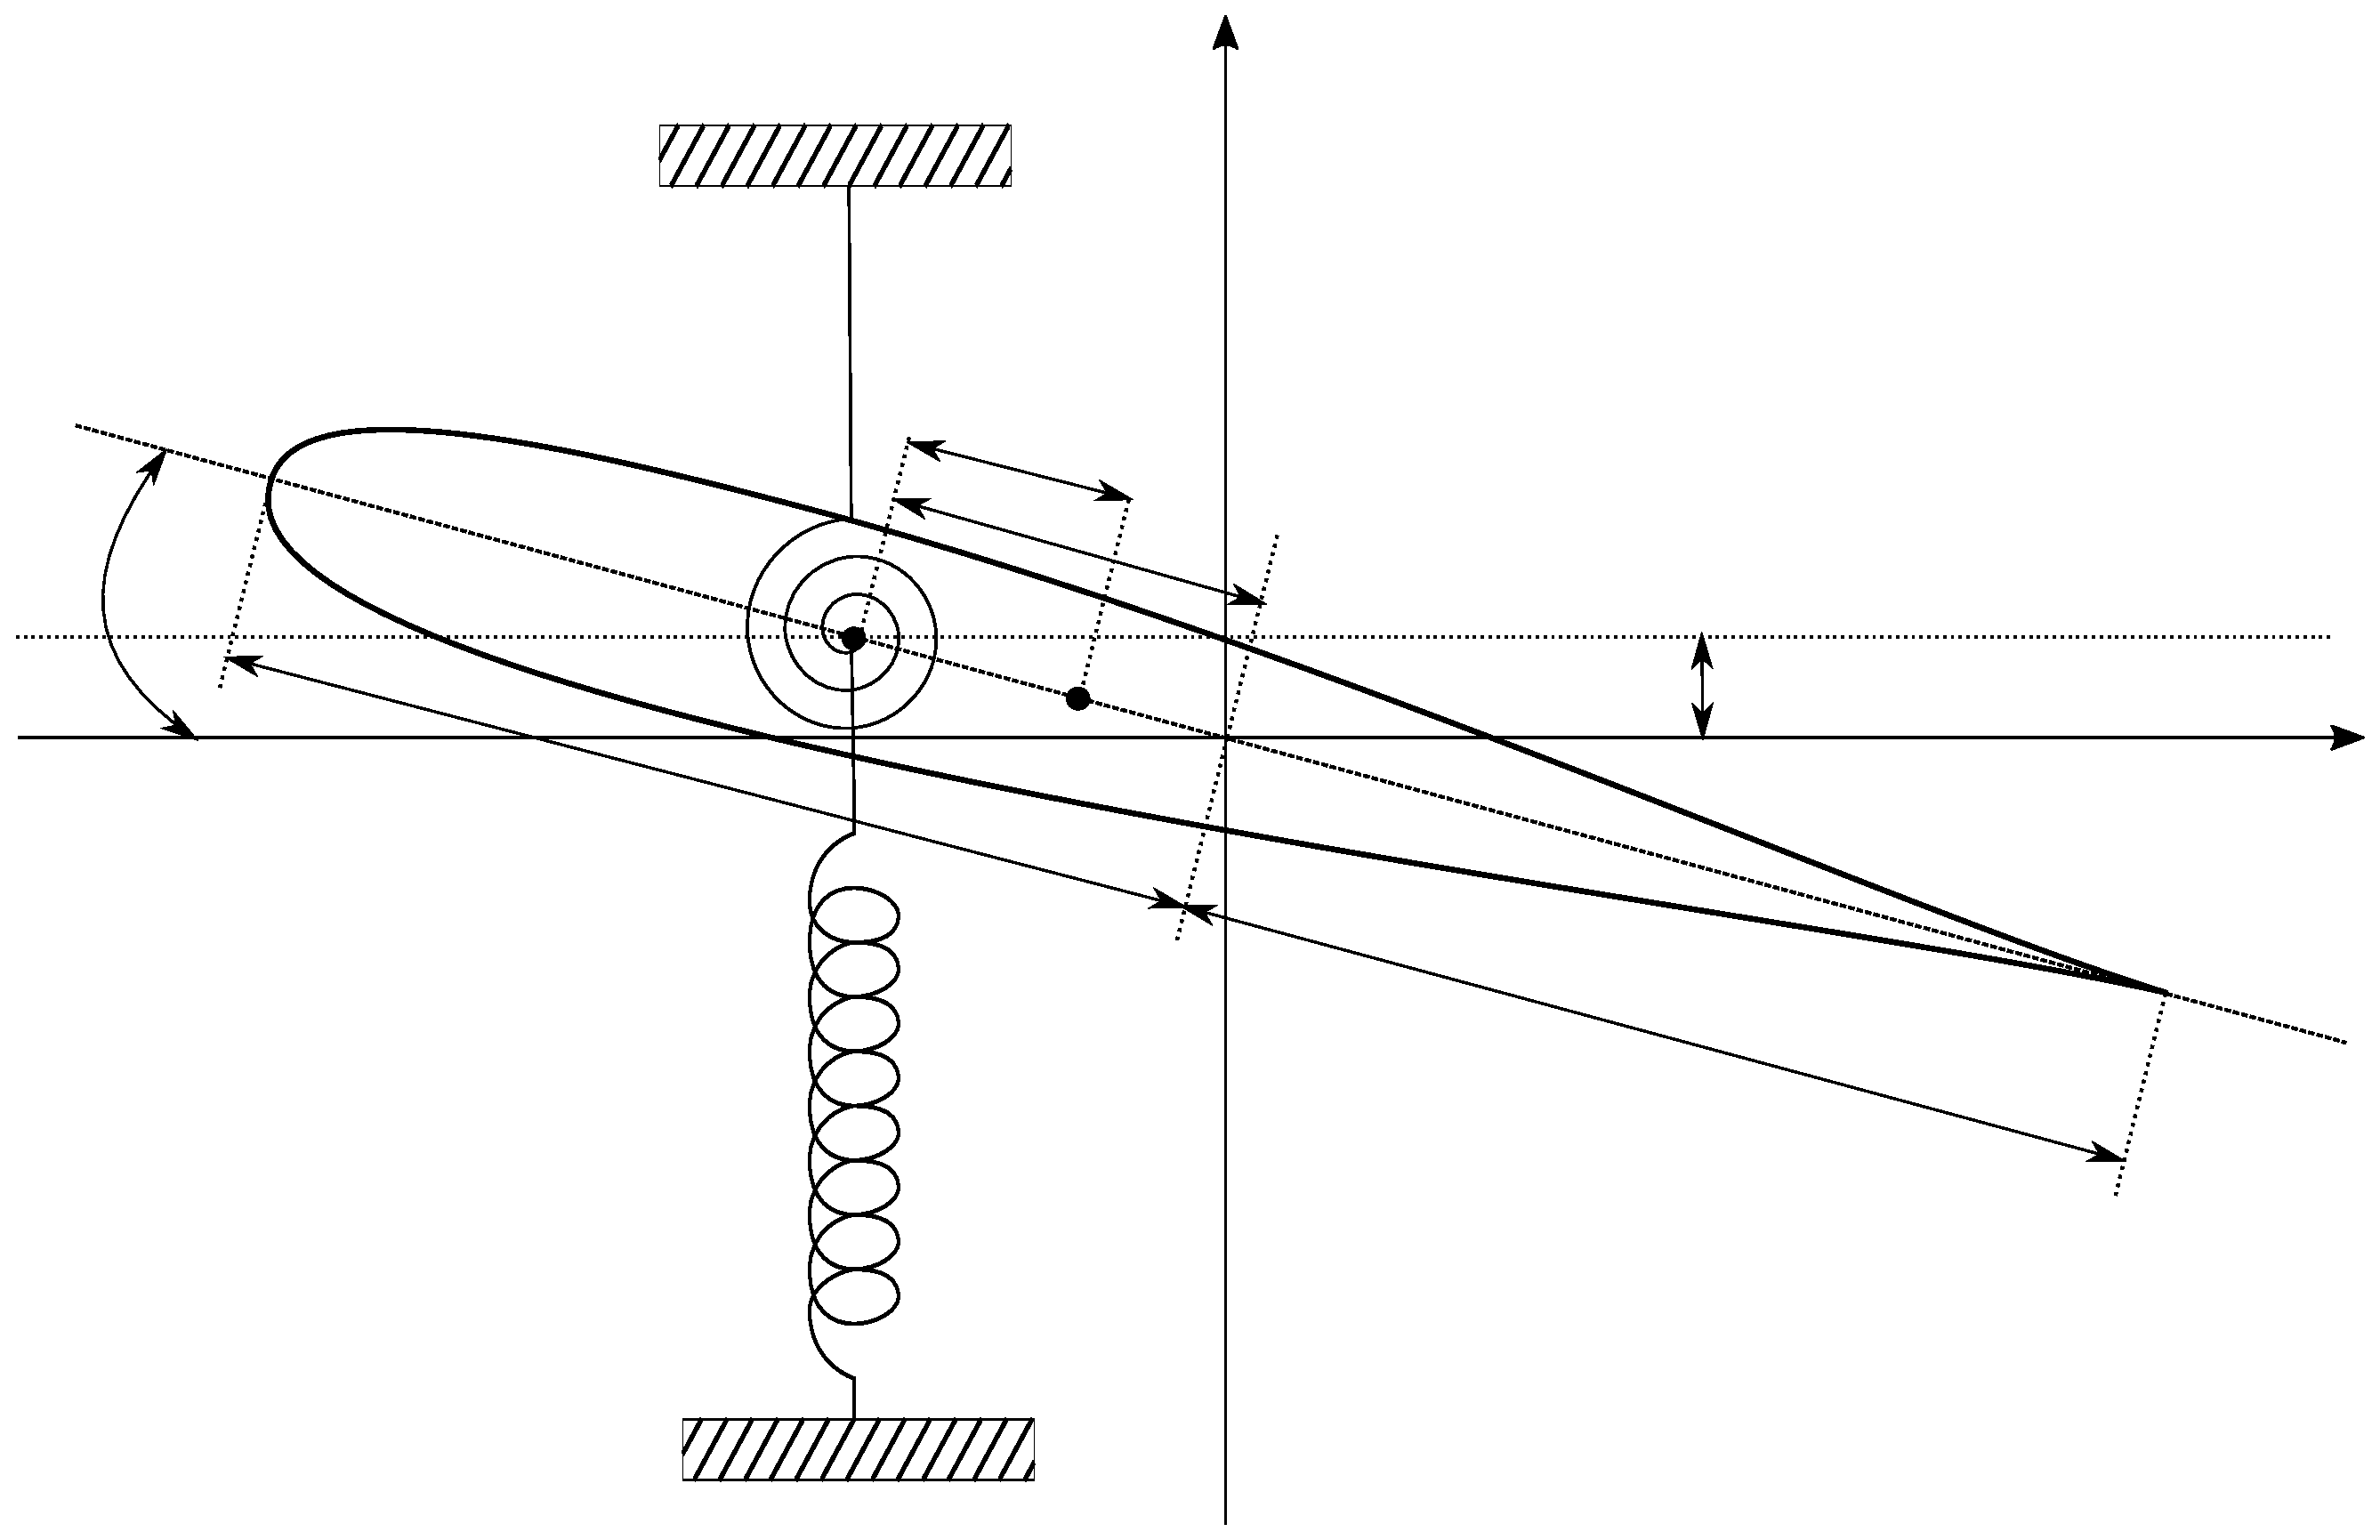
\includegraphics[width=6cm]{flutter_diagram.eps}
  \put(-170,65){$\alpha$}
  \put(-123,45){$b$}
  \put(-60,30){$b$}
  \put(-100,79){$x_{\alpha}$}
  \put(-96,71){$a$}
  \put(-46,58){$h$}
  \caption{Schematic drawing of simplified aeroelastic model.}
  \label{fig:diagram}
\end{figure}

\begin{figure}
  \pgfplotsset{every axis title/.append style={at={(0.5,0.95)}}}
  \begin{tikzpicture}
  \begin{groupplot}[group style={group size=1 by 1,horizontal sep=40pt,every plot/.style={xmin=13,xmax=19,ymin=0,ymax=0.04},xlabels at=edge bottom,vertical sep=30pt},width=10cm,height=5.5cm,xlabel={Wind speed (m/sec)},x label style={at={(0.5,-0.05)}},scatter/classes={%
  		a={mark=*,mark size=2pt,blue},%
  		b={mark=o,mark size=2pt,red}},legend style={at={(0.33,0.95)}},every axis plot/.append style={ultra thick}]

  \nextgroupplot[ylabel={Heave Amplitude (m)},y label style={at={(-0.02,0.5)}}]
          \draw[->] (axis cs:14, 0.014) -- (axis cs:14, 0.005);
          \draw[->] (axis cs:14, 0.016) -- (axis cs:14, 0.018);
          \draw[->] (axis cs:14, 0.035) -- (axis cs:14, 0.02);
          \draw[->] (axis cs:15, 0.012) -- (axis cs:15, 0.005);
          \draw[->] (axis cs:15, 0.015) -- (axis cs:15, 0.02);
          \draw[->] (axis cs:15, 0.035) -- (axis cs:15, 0.023);
          \draw[->] (axis cs:16, 0.010) -- (axis cs:16, 0.005);
          \draw[->] (axis cs:16, 0.013) -- (axis cs:16, 0.022);
          \draw[->] (axis cs:16, 0.035) -- (axis cs:16, 0.026);
          \draw[->] (axis cs:17, 0.0065) -- (axis cs:17, 0.005);
          \draw[->] (axis cs:17, 0.011) -- (axis cs:17, 0.024);
          \draw[->] (axis cs:17, 0.035) -- (axis cs:17, 0.029);
          \draw[->] (axis cs:18, 0.008) -- (axis cs:18, 0.026);
          \draw[->] (axis cs:18, 0.035) -- (axis cs:18, 0.031);
  \addplot [no marks,color=blue]
        table [x=a, y=b, col sep=comma] {./Data/Data_10-2.csv};\label{ps}
  %Here the blue parabloa is defined
  \addplot [no marks,color=red,dashed]
        table [x=a, y=b, col sep=comma] {./Data/Data_10-1.csv};\label{pu}
  \addplot [no marks,color=blue]
        table [x=a, y=c, col sep=comma] {./Data/Data_10-4.csv};
        %Here the blue parabloa is defined
  \addplot [no marks,color=red,dashed]
        table [x=a, y=c, col sep=comma] {./Data/Data_10-3.csv};

  \end{groupplot}
  \end{tikzpicture}
  \centering
\caption{ Bifurcation diagram of unsteady aeroelastic model with physical parameters given in \Tref{t2}. (\ref{ps}) is stable LCO and stable equilibria, (\ref{pu}) is unstable LCO and unstable equilibria. Arrows represents projection of phase portrait near the equilibria and LCO.}
\label{f:TH}
\end{figure}

\section{Control based continuation (CBC)}\label{CBC}

Periodic solution of \Eref{eq:gs} can be tracked via numerical continuation by defining zero problem which has boundary value problem. However, ontinuation of a periodic solution in the experiment needs a different approach with numerical continuation since the equation of motion is unknown. First, the unstable periodic solution should be stabilized by feedback control. The scalar control force $\Gamma(t)$ with proportional derivative control can be expressed as

\begin{align}
  \Gamma(t)=K_p(x^*(t)-x(t))+K_d(\dot x^*(t)-\dot x(t)),
\end{align}

\noindent where $x(t)$ is a scalar output of the system (measured signal), $x^*(t)$ is a scalar control target, $K_p$ is the proportional control gain, and $K_d$ is the derivative control gain. Measuring unstable periodic solution is achieving a noninvasive control which means $\Gamma(t)=0$. Then, controlled system and uncontrolled system has same periodic solution $x(t)$ and the control target $x^*(t)$ is identical to $x(t)$.

$x^*(t)$ that makes the controller noninvasive can be computed from the experiment by solving zero problem defined by input-output map $x^*(t)-x(t)=0$. For instance, input-output map can be discretized by projecting $x^*(t)$ and $x(t)$ to Fourier series of first $2q+1$ modes for the harmonically forced vibrations as

\begin{align}\label{eq:dis}
  \begin{split}
  x(t)=&A_0/2+  \sum_{j=1}^{q} A_j \cos (j\omega t)+B_j \sin (j\omega t),\\
  x^*(t)=&A_0^*/2+  \sum_{j=1}^{q} A^*_j \cos (j\omega t)+B^*_j \sin (j\omega t).
\end{split}
\end{align}

\noindent This expression gives discretized fixed point problem with $2q+1$ equations as

\begin{align}\label{eq:zp}
  \begin{split}
  A_j=&A^*_j \; \textrm{for} \; j=0,1,\ldots,q\\
  B_j=&B^*_j,\; \textrm{for} \; j=1,2,\ldots,q
\end{split}
\end{align}

\noindent \Eref{eq:zp} allows us to define zero problem for multidimensional systems even if we are using scalar input $x^*(t)$ and output $x(t)$ when the feedback control is stabilizing the response. Fixed point problem of CBC can be solved using any zero problem-solving methods such as Newton-like methods \cite{schilder2015experimental} or Picard iteration \cite{barton2013systematic}.

However, stabilizing unstable LCO with CBC is not simple because of the complexity of the input-output map of forced Hopf bifurcation. Zero problem to be solved in the experiment cannot be defined if we use a typical CBC scheme. We will discuss the input-output map of CBC for Hopf bifurcation and define a zero problem in the next section.

\section{Stablizing control near the Hopf bifurcation}\label{SNH}

Simplifying the dynamical system using normal form is the popular way to study the bifurcation problem. There are numerous tools to derive normal form, for example, center manifold reduction, Liapunov-Shmidt reduction and method of multiple scales. In this research, we focus on studying controlled and uncontrolled dynamics near the Hopf bifurcation via center manifold reduction, near-identity transformation, time, and control parameter rescaling. Simplified dynamics of CBC applied to a dynamical system with Hopf bifurcation provides the basis of the developed CBC scheme of this research. Also, we introduce the idea to estimate the unknown parameters from the measured results.

\subsection{Hopf bifurcation and the normal form}\label{SNF}

To simplfy the dynamics, \Eref{eq:gs} should be transformed to a partitioned system at \(\lambda=0\) by transforming the linearization of \(\vec{F}\) to Jordan normal form as
\begin{align}\label{eq:2}
  \begin{split}
    \dot{\vec{x}} =\vec{J}_\textrm{c} \vec{x} + \vec{f}(\vec{x},\vec{y},\lambda)\\
    \dot{\vec{y}} =\vec{J}_\textrm{s} \vec{y} +\vec{g}(\vec{x},\vec{y},\lambda)
  \end{split}
\end{align}
where $\lambda \in \real ^m$ is the control parameter vector, $\vec{x}=[x;\bar{x}]\in \complex^2$ is center subspace with associated Jordan matrix $\vec{J}_\textrm{c}$ having diagonal term $\pm\textrm{i}$ and $\vec{y}\in \complex^{n-2}$ is stable subspace with it's associated Jordan matrix $\vec{J}_\textrm{s}$ of Jacobian of $\vec{F}(\vec{z})$ at $\vec{z}=0$.
$\vec{f}$ and $\vec{g}$ are functions with $\vec{f}(0,0)=0$, $D\vec{f}(0,0)=0$ and $\vec{g}(0,0)=0$, $D\vec{g}(0,0)=0$. Centermanifold exists for dynamical system \Eref{eq:2} for small  $\|\vec{x}\|$ which is invariant under the action of dynamical system \cite{carr2012applications}. Note that eigenvalues corresponding to center subspace is assumed $\pm\textrm{i}$ for simplicity. To reduce the order of dynamics of Hopf bifurcation, we include $\dot\lambda=0$ to \Eref{eq:2} and analyze the family of center manifolds, locally represented by small $\|\lambda\|$  \cite{kuznetsov2013elements}. Power series of centermanifold $\vec{H}(\vec{x},\lambda)$ can be computed recursively by solving
\begin{align}\label{eq:3}
    D\vec{H}({\vec{\hat{x})}}(\vec{\hat{J}}_\textrm{c}\vec{\hat{x}}+\vec{f}(\vec{\hat{x}},\vec{H}(\vec{\hat{x}}))) =\vec{J}_\textrm{s} \vec{H}(\vec{\hat{x}})-\vec{g}(\vec{\hat{x}},\vec{H}(\vec{\hat {x}}))
\end{align}
at each order of power series, where \(\vec{\hat{x}}=[\lambda;\vec{x}]\) and \(\vec{\hat{J}}_c\) is the extended Jordan matrix which zero eigenvalue is added to \(\vec{J}_\textrm{c}\). Then, we can compute the reduced dynamics on the centermanifold as a power series which will have a form as
\begin{align}\label{eq:4}
  \begin{split}
    {}&\dot{x} =\textrm{i} x+\sum_k f_k(x,\bar{x},\lambda)\\
    ,\textrm{where} \; & f_k=\sum_{j+l+m=k}(\vec{a}_{1jlm}+\textrm{i}\vec{a}_{2jlm})x^j\bar{x}^l\lambda^m.
  \end{split}
\end{align}
Note that in \Eref{eq:4}, \(\lambda=[\lambda_1;\lambda_2;\ldots;\lambda_m]\) and \(\lambda^m\) denotes \(\lambda_1^{m_1}\lambda_2^{m_2}\cdots\lambda_m^{m_m}\) satisfying \(\sum_i m_i = m\) with \(\vec{a}_{1jlm}=[a_{1jlm_1};a_{1jlm_2};\ldots;a_{1jlm_m}]\).

Recently, researchers have worked extensively to develop an efficient simplest normal form of Hopf bifurcation using computer algebra \cite{yu1998computation}. Simplest normal form (SNF), simplest means that the number of terms retained at each order of is minimized, is one of the most effective ways to derive the normal form from the nonlinear differential equation defined on center manifold. We can derive third order polynomial of amplitude in polar coordinates where conventional normal form has infinite degree high order terms. Moreover, we can parametrize amplitude and the stability of LCO by parameters of the original coordinate system if we use SNF. Unlike the dynamical system without control parameters, SNF cannot be computed using only near identity transformation. P.Yu \cite{yu2002simplest} proved time and parameter rescaling is essential additional to near identity transformation and developed a recursive formula to compute SNF up to $k$-th order as
\begin{align}\label{eq:5}
  \begin{split}
    &\frac{du}{d\tau}=(\vec{\alpha}_1 \nu+\textrm{i}\vec{\beta}_1) u+(\vec{\alpha}_2+\textrm{i}\vec{\beta}_2) u^2 \bar{u}+\textrm{i}\sum_k g_k(u,\bar{u}),\\
    \textrm{where} \;  &g_k(u,\bar{u})=(b_{1k}+\textrm{i}b_{2k})u^{\frac{k+1}{2}}\bar{u}^{\frac{k-1}{2}}, \; \textrm{for odd integer} \;k \geq 5.
  \end{split}
\end{align}
Here, \(\vec{u}=[u,\bar{u}]\) and equation of complex conjugate variable \(\bar{u}\) is neglected. \(u\),\(\tau\) and \(\nu\) are transformed from \(x\),\(t\) and \(\lambda\) by near identity transformation
\(x=h(u,\bar{u},\nu))=u+\sum_k h_k(u,\bar{u},\nu)\), time rescailing \(t=T(u,\bar{u},\nu,\tau)\) and parameter rescailing \(\lambda=p(\nu)\). More detailed explanation on the derivation and coefficients $\alpha_1$, $\alpha_2$, $\beta_1$, and $\beta_2$ and function $h$, $T$, $g$ and $p$ is presented in \cite{yu2002simplest}.

If we express \Eref{eq:5} in polar coordinates $u=Re^{\textrm{i}\theta}$ and collect the real part, following equation can be derived as

\begin{align}\label{eq:polar}
  \begin{split}
    &\frac{dR}{d\tau}=\vec{\alpha}_1 \nu R+\vec{\alpha}_2 R^3,
  \end{split}
\end{align}

\noindent where the nonzero fixed point of \Eref{eq:polar} is the amplitude of the LCO.

\subsection{Stabilizability of the controller}

We will consider linear proportional derivative control acting on a single coordinate vector which is a convenient setup a nonlinear dynamic experiment. Let the equation of motion of autonomous dynamical system that has  generic subcritical Hopf bifurcation at $\mu=0$ be

\begin{align}\label{eq:0}
    \dot{\vec{z}} =\vec{G}(\vec{z},\vec{\mu}).
\end{align}

\noindent where $\mu\in \real$ is an unfolding parameter of uncontrolled system, and $z_{j+1}=\dot z_j$ for all odd $j$. To stabilize the unstable periodic orbit near the Hopf bifurcation point, we add a proportional derivative feed-back control to \Eref{eq:0}. Let us assume that the control force is applied in the direction of the one principle coordinates to \Eref{eq:0} as

\begin{align}\label{eq:11}
    \dot{\vec{z}} =\vec{G}(\vec{z},\vec{\mu})+\vec{e}_{j+1}(K_p(z^*(t)-z_j)+K_d(\dot z^*(t)-z_{j+1})),
\end{align}

\noindent where $\mu\in \real$ is an control parameter of uncontroled system, $\vec{e}_{j+1}$ is $j+1$ th standard basis, $z_{j}$, $z_{j+1}$ are monitored signal for the control, and $z^*(t)$  is the time-periodic control target. We will show the controlled system can be simplified to forced Hopf bifurcation where the single harmonic forcing is added to a SNF of the unforced equation under a certain assumption. We can understand more easily how CBC can stabilize the unstable LCO near the Hopf bifurcation point if \Eref{eq:11} is simplified to a normal form.

First, we analyze unforced term of \Eref{eq:11} by dropping off the time-periodic forcing $\vec{e}_{j+1}(K_p(z^*(t))+K_d(\dot z^*(t)))$ as

\begin{align}\label{eq:12}
    \dot{\vec{z}} =\vec{G}(\vec{z},\vec{\mu})-\vec{e}_{j+1}(K_p z_j+K_d z_{j+1}).
\end{align}

\noindent \Eref{eq:12} can be written in the form of \Eref{eq:gs} by

\begin{align}\label{eq:13}
\begin{split}
  F({\vec{z}})=&\vec{G}(\vec{z},\vec{\mu})-\vec{e}_{j+1}(K_pz_j+K_d z_{j+1})\\
  \lambda=&[\mu,K_p,K_d]^T.
\end{split}
\end{align}

\noindent As explained in \Ssref{SNF}, we can derive the reduced dynamics on center manifold of \Eref{eq:13} and compute SNF using nonlinear transformation between center subspace of origianl coordinates $[x,\bar x]^T$ and normal form coordinates $[u,\bar u]^T$ and rescailing time and control parameters.

Now, stability of LCO of the uncontroled system can be studied from normal form of \Eref{eq:12} at $\lambda=\lambda_1=[\mu,0,0]^T$. LCO ($[u_1(\tau),\bar u_1(\tau)]^T$) is a nonzero fixed point of \Eref{eq:polar} and expressed in normal form coordinates $[u,\bar u]^T$ as

\begin{align}\label{eq:14}
  \begin{split}
      u_1(\tau)=&R_1e^{\textrm{i}\omega_1 \tau},\\
      \bar u_1(\tau)=&R_1e^{-\textrm{i}\omega_1 \tau},
    \end{split}
\end{align}

\noindent where $R_1$ is the amplitude and $\omega_1$ is frequency of the limit cycle in rescailed time. If we define homeomorphism($\Psi_1:\complex\times\complex\rightarrow\complex\times\complex$) between the original coordinates $[x,\bar x]^T$ and normal form coordinates $[u,\bar u]^T$ at $\lambda=\lambda_1$ as

\begin{align}\label{eq:15}
    [x,\bar x]^T=\Psi_1(u,\bar u)=&[h(u,\bar u,\nu_1),\bar h(u,\bar u,\nu_1)]^T,
\end{align}

\noindent  where $\nu_1=p^{-1}(\lambda_1)$ is control parameter reparametrization in the coordinates of the normal form with $p(0)=0$. Limit cycle \Eref{eq:14} in original coordinates $x^*(t)$ can be computed from

\begin{align}\label{eq:16}
    [x^*(\tau),\bar {x^*}(\tau)]^T=\Psi_1(R_1e^{\textrm{i}\omega_1 \tau},R_1e^{-\textrm{i}\omega_1 \tau}).
\end{align}

\noindent If we define \textbf{Noninvasive periodic solution} as a periodic solution of \Eref{eq:11} where control force $\vec{e}_{j+1}(K_p(z^*(t)-z_j)+K_d(\dot z^*(t)-z_{j+1}))$ is zero, noninvasive periodic solution of \Eref{eq:11} is solution of \Eref{eq:0} since $\vec{e}_{j+1}(K_p(z^*(t)-z_j)+K_d(\dot z^*(t)-z_{j+1}))=0$. Moreover, by assuming $\| \lambda \|$ is small enough to say periodic solution near the equilibria of \Eref{eq:13} is on the center manifold, we can derive the following lemma which relates the control target and the noninvasive periodic solution.

\begin{lemma}\label{l1}
$\vec{z}(t)=\vec{\Sigma}[x^*,\bar {x^*},\vec H(x^*,\bar {x^*},\lambda)]^T$ is a noninvasive periodic solution of \Eref{eq:11} if and only if $z^*(t)=\pi_j \vec{\Sigma}[x^*,\bar {x^*},\vec H(x^*,\bar {x^*},\lambda)]^T$,
where $\vec{\Sigma}$ is a coordinate transformation matrix to jordan normal matrix $\vec{J}$ satisfying $\vec{J}=\Sigma^{-1}\vec{F}_\vec{z}(0,\lambda) \Sigma$ at $\lambda=0$, and $\pi_j$ is a scalar projection to j-th principle coordinate.
\end{lemma}

\begin{proof}
If $z^*(t)=\pi_j \vec{\Sigma}[x^*,\bar {x^*},\vec H(x^*,\bar {x^*},\lambda)]^T$, by inserting $\vec z(t)=\vec{\Sigma}[x^*,\bar {x^*},\vec H(x^*,\bar {x^*},\lambda)]^T$ to \Eref{eq:11}, we have $\vec{G}(\vec{z},\mu)=0$ and the control force is zero. For the only if part, let $z(t)=\vec{\Sigma}[x^*,\bar {x^*},\vec H(x^*,\bar {x^*},\lambda)]^T$ is a noninvasive periodic solution. Then, $z^*(t)=\pi_j z(t)$ from noninvasiveness.
\end{proof}

\noindent Let $\lambda_2=[\mu,K_p,K_d]^T$ and stability of the noninvasive periodic solution with control target defined as \Lref{l1} at $\lambda=\lambda_2$ will be analyzed. We make the following assumption on the near identity transformation and amplitude $R_1$ to develop a scheme that is practically applicable in experiments.

\begin{assumption}\label{a1}
For $\lambda=\lambda_1$ and $\lambda=\lambda_2$, $c_{1jlm}\nu^m$, $c_{2jlm}\nu^m$ in \Eref{eq:6} is sufficiently small, and therefore neglectable for $j+j+m\geq 2$, i.e., $x \approx u$. Also, $R_1$ is small enough to have $t=T(u_1,\bar u_1,\tau) \approx \tau$ and $\vec H(x^*,\bar {x^*},\lambda) \approx 0$.
\end{assumption}

\noindent  Under \asref{a1}, periodic solutions in the normal form will be transformed into a single harmonic oscillator in the original coordinates. Therefore, limit cycle in original coordinates $x^*(t)$ and control target  $z^*(t)$ can be expressed as a single harmonic oscillator with small amplitude by using the result of \Lref{l1}. Now, our problem to be solved is Hopf bifurcation with single harmonic forcing. The normal form of forced Hopf bifurcation for small amplitude bounded solution is equivalent to adding force in the direction of the center subspace to the autonomous Hopf normal form (see \cite{golubitsky2012feed,elphick1987normal} for the proof). We assume $\| \vec{e}_{j+1}(K_p(z^*(t))+K_d(\dot z^*(t)))\|$ is sufficiently small to have solutions of \Eref{eq:11} on the center manifold. Then, by letting $\epsilon$ as an amplitude of periodic forcing which is appropriately rescailed by projecting $\vec{e}_{j+1}(K_p(z^*(t))+K_d(\dot z^*(t)))$ to the center subspace, SNF of \Eref{eq:11} at $\lambda=\lambda_2$ can be derived as

\begin{align}\label{eq:18}
  \frac{du}{dt}=(\alpha_1 \nu_2+\textrm{i}\beta_1)u+(\alpha_2+\textrm{i}\beta_2)u^2\bar u+\epsilon e^{\textrm{i}\omega_1 t},
\end{align}

\noindent where coefficients $\alpha_1$, $\alpha_2$, $\beta_1$, and $\beta_2$ can be computed from the coefficients of reduced dynamics at the centermanifold at $\lambda=\lambda_2$, and $\nu_2$ is the rescailed control parameter vector satisfying $\lambda_2=p(\nu_2)$. Stabilizability of the controller can be anlyzed by the stability of the noninvasive periodic solution of \Eref{eq:18} $u=u_2(t)$. Under \asref{a1}, noninvasive periodic solution can be expressed as $u_2(t)=R_1e^{\textrm{i}\omega_1 t}$,  and the stability condition can be derived as following lemma.

\begin{lemma}\label{t1}
Noninvasive periodic solution $u_2(t)$ is stable if the amplitude of the noninvasive periodic solution $R_1$ satisfies
\begin{align}\label{eq:20}
3(\alpha_2^2+\beta_2^2)R_1^3+4(\alpha_1 \nu_2+\beta_2(\beta_1-\omega_1))R_1+((\alpha_1 \nu_2)^2+(\beta_1-\omega_1)^2)<0.
\end{align}
\end{lemma}

\begin{proof}
If we look \Eref{eq:18} in the rotating coordinates defined by

\begin{align}\label{eq:21}
  v=ue^{\textrm{i}\omega_1 t},
\end{align}

\noindent The dynamical system becomes autonomous,

\begin{align}\label{eq:22}
  \dot v=(\alpha_1 \nu_2+\textrm{i}(\beta_1-\omega_1))v+(\alpha_2+\textrm{i}\beta_2)v^2\bar{v}+\epsilon.
\end{align}

\noindent $v$ satisfying $\dot v=0$ is a phase-locked periodic solution with the forcing of \Eref{eq:18}. We obtain algebraic equation by setting $\dot v=0$ and $R=|v|$,

\begin{align}\label{eq:23}
  ((\alpha_1\nu_2+\alpha_2R^2)+\textrm{i}((\beta_1-\omega_1)+\beta_2 R^2)))v=-\epsilon.
\end{align}

\noindent $P(R)$, where the zeros of $P(R)$ is phase-locked periodic solutions of \Eref{eq:18}, can be derived by taking norm square of both side of \Eref{eq:23} as

\begin{align}\label{eq:24}
  P(R)=(\alpha_2^2+\beta_2^2)R^6+2(\alpha_1 \nu_2+\beta_2(\beta_1-\omega_1))R^4+((\alpha_1 \nu_2)^2+(\beta_1+\omega_1)^2)R^2-\epsilon^2=0.
\end{align}

\noindent Since the noninvasive periodic solution is phase-locked solution of \Eref{eq:18} at $R=R_1$ which is a non-zero fixed point of $P(R)$ which is stable if $P_R(R_1)<0$. Therefore, dividing $P_R(R_1)$ by $2R_1^2$, we arrive to the stability condition of the noninvasive periodic solution.
\end{proof}

\noindent From \Lref{t1}, we can see the stability of noninvasive periodic solution depends on parameters of the original dynamical system, including amplitude and frequency of LCO, and control parameters $\mu$, $K_p$, and $K_d$. The controller can stabilize the unstable LCO of the uncontrolled system if the noninvasive periodic solution is stable. Also, it is interesting to see that the feedback controller is able to stabilize the unstable LCO even if the control force is applied to an arbitrary direction, given the amplitude of the response is small. In fact, the proposed CBC method works sufficiently well, even in high amplitude responses. However, $z^*(t)$, and suitable control gains $K_p$, $K_d$ to stabilize the noninvasive periodic solution is unknown factors for CBC experiments. Implementing CBC experiment to stabilize the unstable LCO is generally finding $z^*(t)$ from the experiment with suitable $K_p$, and $K_d$ that makes controller noninvasive. The scheme for solving this problem will be discussed in the next subsection.

\subsection{Scheme for finding noninvasive periodic solution}\label{FNP}

In general experiment, stabilizability of the control cannot be determined from the equation as in \Sref{SNF}. We will discuss effective scheme to find noninvasive periodic solutions near the Hopf bifurcation in this subsection.

Phase-locked response with the forcing should be tracked from the response of forced Hopf bifurcation, see \cite{zhang2011periodically,wiser2015bifurcations} for detailed bifurcation diagram, to find the noninvasive periodic solution. However, solutions of \Eref{eq:20} are not necessarily to be in phase with forcing frequency. For example, if we set rotating coordinates of \Eref{eq:21} $v=ue^{\textrm{i}(\omega_2 \tau-\theta)}$, where $\theta$ is an arbitrary phase shift, we can rewrite \Eref{eq:18}
as

\begin{align}\label{eq:ps}
\dot v=(\alpha_1+\textrm{i}\beta_1)v+(\alpha_2+\textrm{i}\beta_2)v^2 \bar v+\epsilon e^{\textrm{i}\theta}.
\end{align}

\noindent A stationary solution of \Eref{eq:ps} with arbitrary phase shift $\theta$ is also a periodic response of the controlled system. This phase shift of the response and control target depends on initial condition, which is uncontrollable. Therefore, it makes the problem much simpler if we can force the response to be in phase with a control target to determine the noninvasive periodic solution.

We use a phase plane based CBC (PP-CBC) to achieve phase locking between target coefficients $z^*(t)$ with the response in \Eref{eq:11}. This is equivalent to phase-locking between force and response in \Eref{eq:20}, which was first proposed in \cite{irene}. Monitored signals $z_j$, $z_{j+1}$  are assumed as an analytic signal,

\begin{align}\label{eq:25}
\begin{split}
z_{j}(t)=&A(t)\cos{\phi},\\
z_{j+1}(t)=&-\dot\phi A(t)\sin{\phi}
\end{split}
\end{align}

\noindent where $A(t)$ is the instantaneous amplitude, $\phi$ is the instantaneous phase of the response, $\dot\phi$ is the frequency of the response which is constant if the system is at the steady-state. If we set target coefficient as

\begin{align}\label{eq:26}
z^*(t)=\hat A\cos\Big(\tan^{-1}\Big({\frac{-z_{j+1}(t)}{ \dot \phi z_{j}(t)}}\Big) \Big),
\end{align}

\noindent where $\hat A$ is the amplitude of the control target, phase of the target is locked with the response since single harmonic response is assumed. Specifically, phase is locked by updating $\dot\phi$ every fixed time interval from the measurement and wait until the system reaches the steady-state. This phase-locked condition is equivalent to $\dot v=0$ in \Eref{eq:22} and as a result control target has a form:

\begin{align}\label{eq:tg}
 z^*(t)=\hat A\cos{\phi}.
\end{align}

\noindent Moreover, final steady-state response is the fixed point of $P(R)$ in normal form coordinates if $P_R<0$ with $\epsilon=\epsilon(\hat A)$. Now, zero problem can be derived from input output map which is defined as a one-dimensional function of $\hat A$ by control error $\Xi=\hat A - A(\hat A)$ where $A$ is amplitude of the response in original coordinates. We can say the controller is stabilizable if the sequence of control error $\Xi_k=\hat A_k-A_k$ crosses zero for some $\hat A_k$ with step size $\Delta_k=\hat A_{k+1}-\hat A_{k}$.

Let us say we found a zero-crossing sequence of $\Xi_k$ from the experiment, which means the controller is stabilizable. Then, finding a noninvasive periodic solution is equivalent to finding  $|\Xi_k|<\delta$, where $\delta$ is the zero-tolerance. The noninvasive periodic solution can be found by decreasing the stepsize $|\Delta_k|=|\Delta_{k-1}|/2$ and changing the searching direction whenever $\Xi_k$ crosses zero. The procedure to find zero error is summarized in \Fref{f:1}.

\begin{figure}
\tikzstyle{decision} = [diamond, draw, fill=blue!20,
    text width=7em, text badly centered, inner sep=0pt, minimum height=3em]
\tikzstyle{decision2} = [diamond, draw, fill=blue!20,
        text width=6em, text badly centered, inner sep=0pt, minimum height=3em]
\tikzstyle{block} = [rectangle, draw, fill=blue!20,
    text width=8em, text centered, rounded corners, minimum height=4em]
\tikzstyle{block2} = [rectangle, draw, fill=blue!20,
        text width=13em, text centered, rounded corners, minimum height=3em]
\tikzstyle{block3} = [rectangle, draw, fill=blue!20,
                text width=8em, text centered, rounded corners, minimum height=3em]
\tikzstyle{block4} = [rectangle, draw, fill=blue!20,
                text width=4em, text centered, rounded corners, minimum height=3em]
\tikzstyle{line} = [draw, -latex']
\tikzstyle{cloud} = [draw, ellipse,fill=red!20, node distance=3cm,
    minimum height=2em]

\begin{center}
\begin{tikzpicture}[node distance = 2cm, auto]
    % Place nodes
    \node [block4] (init) {$\hat A=\hat A_k$};
    \node [block2, below of=init,node distance=1.3cm] (identify) {Wati until system reaches steady state};
    \node [decision2, below of=identify,node distance=1.9cm] (evaluate) {$|\Xi_k|<\delta$};
    \node [block4, left of=evaluate, node distance=4cm] (update) {stop};
    \node [decision, below of=evaluate,node distance=2.7cm] (decide) {$|\Xi_k||\Xi_{k-1}|<0$};
    \node [block3, left of=decide, node distance=4cm] (update2) {$\Delta_k=-\Delta_{k-1}/2$};
    \node [block, below of=decide, node distance=2.3cm] (stop) {$\Delta_k=\Delta_{k-1}$\\ $\hat A_{k+1}=\hat A_k+\Delta_k$ \\$k=k+1$};
    % Draw edges
    \path [line] (init) -- (identify);
    \path [line] (identify) -- (evaluate);
    \path [line] (evaluate) -- node {no} (decide);
    \path [line] (evaluate) -- node [near start] {yes} (update);
    \path [line] (decide) -- node [near start] {yes} (update2);
    \path [line] (decide) -- node {no}(stop);
    \path [line] (update2) |- (stop);
    %  \path [line] (stop.east) [xshift=5em] -- (init.east);
      \path[line] (stop.east) -- (4,-8.2) --(4,0)
   --(init.east);

\end{tikzpicture}
\end{center}
\centering
\caption{Flow chart diagram of finding noninvasive periodic solution}
\label{f:1}
\end{figure}

\subsection{Parameters estimation from the CBC results}\label{NSI}
CBC results can be used as a tool of system identification if we have a model \Eref{eq:0} and identified parameters associated with the linearization of \Eref{eq:0}. Periodic solutions of \Eref{eq:0} can be computed numerically if the periodic boundary value problem is defined. Periodic boundary value problem can be transformed to a system of nonlinear equations where the unknown variables are period of LCO, and the grid points of the periodic solution if spectral method is used (see \cite{trefethen2000spectral} for detail). Results of the normal form computation provides good initial point of solving nonlinear equations derived from the periodic boundary value problem. Then, we can use the solution of the periodic boundary value problem $z(\mu_M,\theta_n)$, where $\theta_n$ is parameter vector associated with the nonlinear part of the \Eref{eq:0} and $M$ is the index of the measurement, to define the prediction error function $\hat{V}(\theta_n)$ as

\begin{align}\label{NSI-2}
\hat{V}(\theta_n)= \sum_M (|\pi_j z(\nu_M,\theta_n)|-|(z_j)_M|)^2,
\end{align}

\noindent where $(z_j)_M$ is $M$-th measurement result from CBC experiment and absolute sign denotes the amplitude of the periodic response. Note that sign of $\alpha_2$ in \Eref{eq:polar} characterizes the type of the bifurcation which can provide a constraint to a parameter estimation problem. For subcritical Hopf bifurcation, $\theta_n$ can be identified by solving optimization problem to minimize the prediction error function $\hat{V}(\theta_n)$.

\begin{align}\label{NSI-3}
\hat{\theta_n}=&\underset{\theta_n \: \textrm{s.t.} \: \alpha_2>0} {\arg\min} \: \hat V(\theta_n).
\end{align}

\section{CBC experiment and system identification}
In this section, we show a scheme developed in \Sref{SNH} can be applied to a mechanical system with Hopf bifurcation. The developed scheme is applied to a flutter rig, and we present the methodology to estimate the parameters of the mathematical model.

\subsection{Experimental setup and mathematical model}\label{model}
\subsubsection{Experimental rig and settings}\label{setup}
The experiment was performed on a flutter rig with a NACA-0015 wing profile \cite{jacobs1933characteristics}. The profile moves in two degrees of freedom, heave, and pitch. Coil springs are installed to add linear stiffness to the heave and pitch motion, and spring plate is installed to add nonlinearity on the pitch stiffness. Measurements are taken at shaft with digital encoder for pitch and heave motion was measured from laser displacement sensor.

Developed CBC scheme in this paper runs on a laptop computer connected to the real-time controller (RTC). The RTC box consists of a BeagleBone Black on which is fitted with a custom data acquisition board \cite{rtc2} in which the real-time feedback controller used in CBC is implemented. Measurements are taken with sampling frequency  5kHz without any filter.  Control force was applied to heave motion to stabilize unstable LCO with APS Electro-Seis Shaker and schematics of a configuration of the experiment and picture of the rig is presented in \Fref{f:rig}.

\begin{figure}
  \centering
  \begin{subfigure}[b]{0.5\linewidth}
    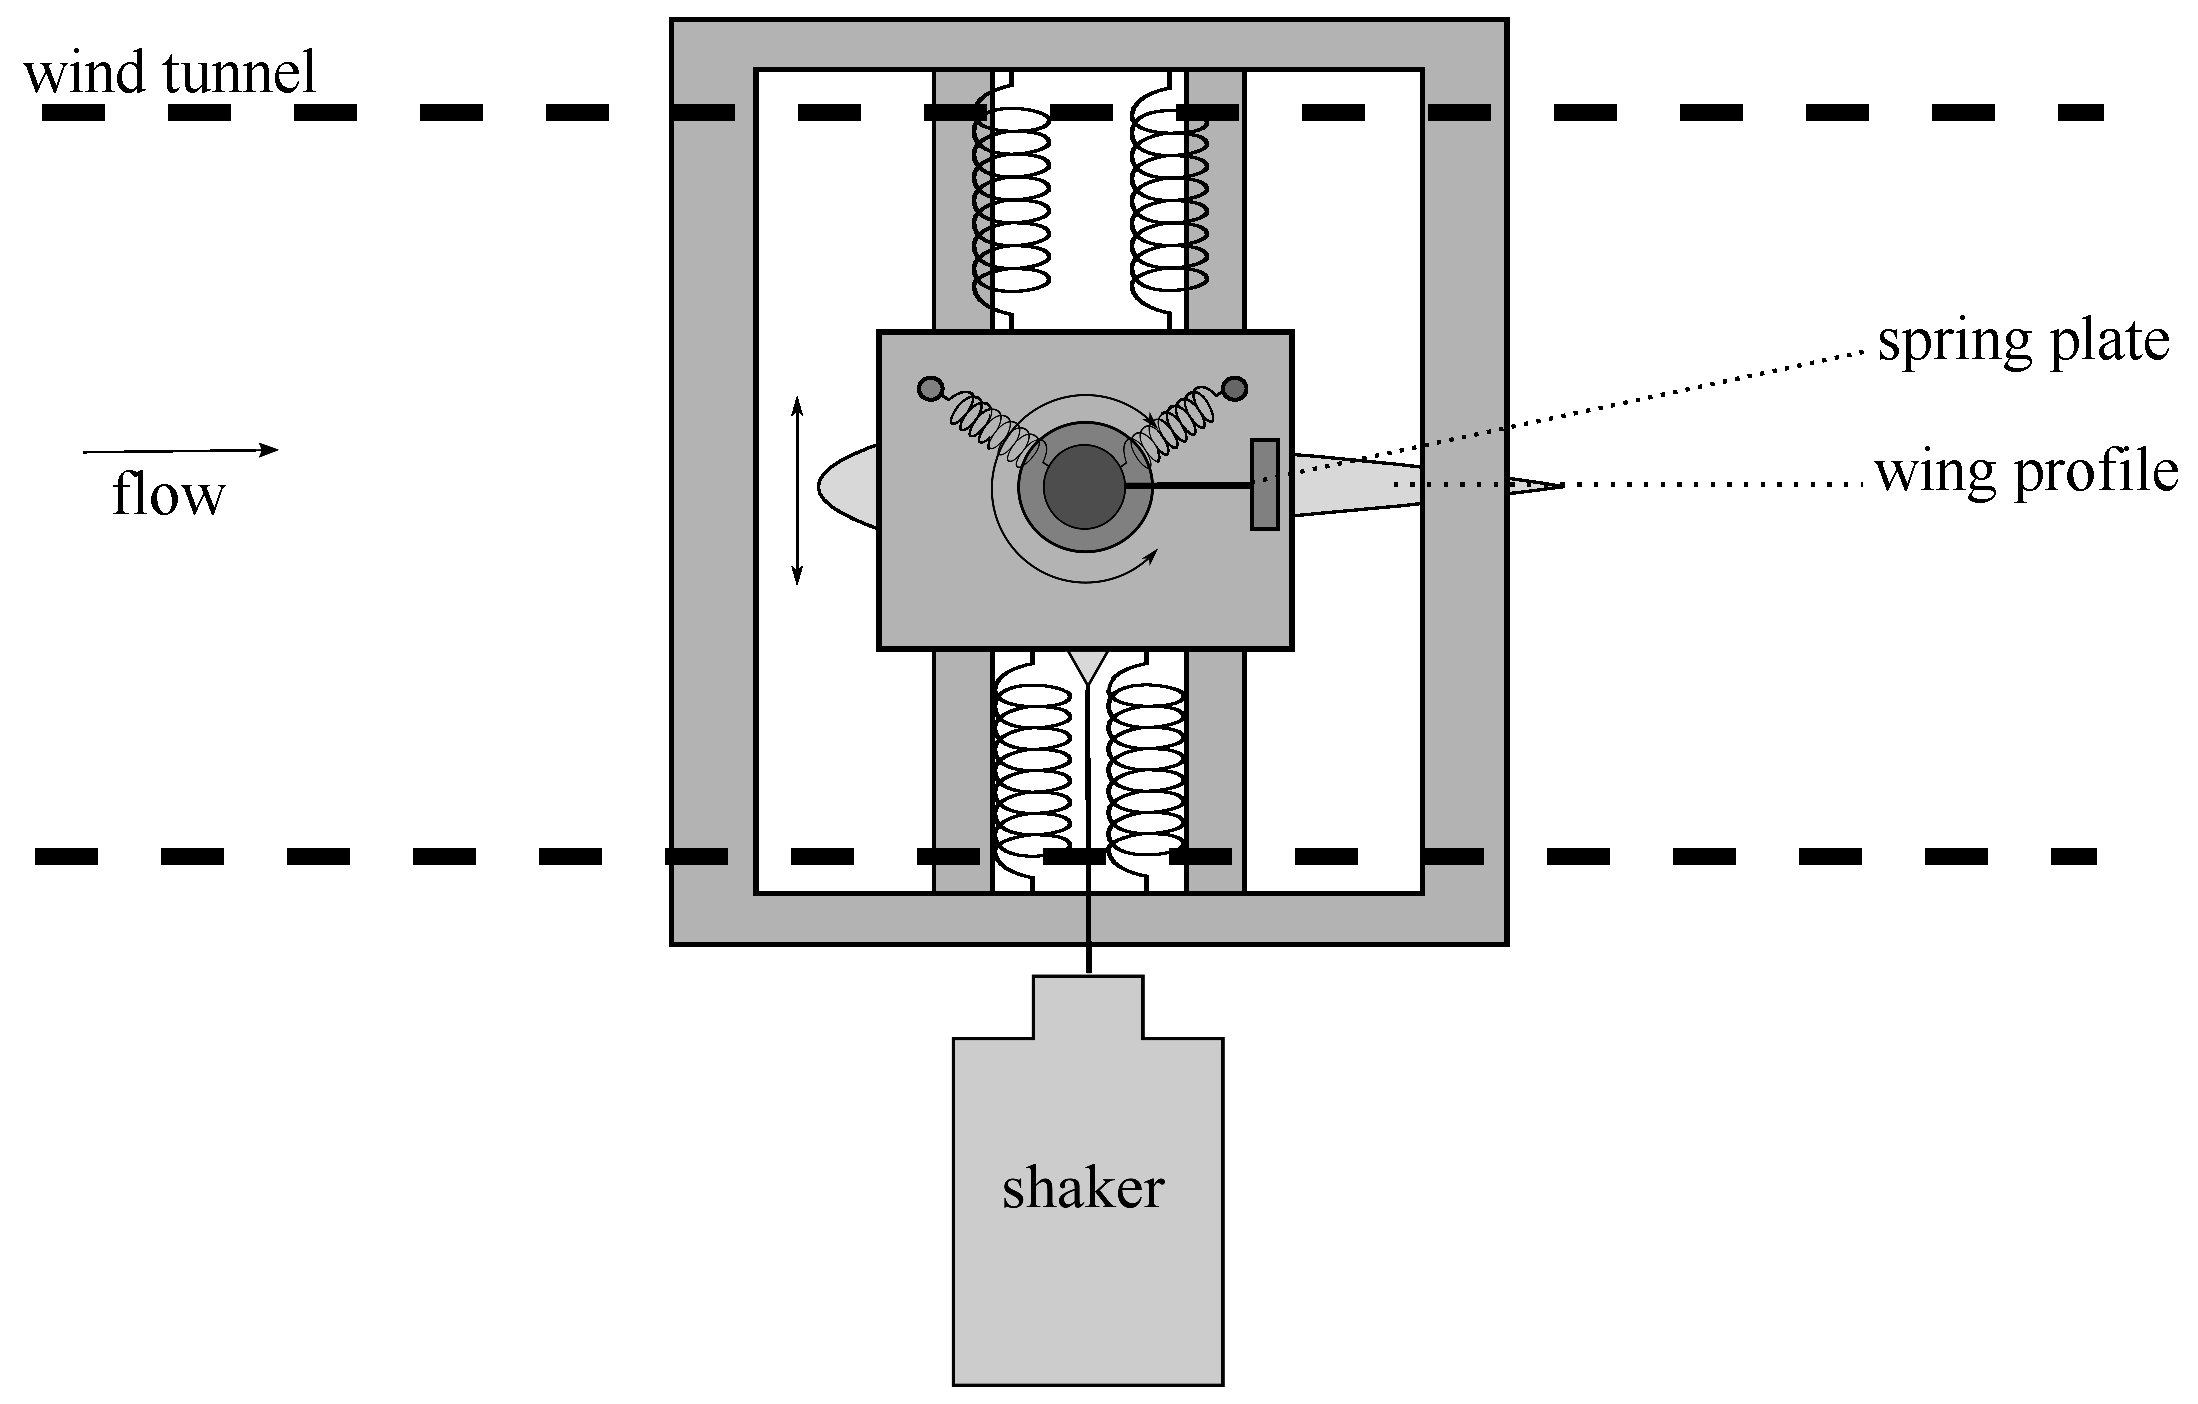
\includegraphics[width=\linewidth]{flutter_rig.eps}
    \caption{Schematic of flutter rig}
  \end{subfigure}
  \begin{subfigure}[b]{0.45\linewidth}
    \includegraphics[width=\linewidth]{rig_pic.png}
    \caption{Picture of flutter rig.}
  \end{subfigure}
  \caption{Schematic drawing and picture of flutter rig.}
  \label{f:rig}
\end{figure}

\subsubsection{Mathematical model}\label{Math_model}
There are many physical models describing flutter; however, we use a simplified 2D model since the wing profile of the flutter rig has a simple shape. To take account of wake effects on the aerodynamic loads, we use unsteady formulation \cite{abdelkefi2013analytical}, which is more accurate compared to quasi-static model \cite{strganac2000identification}. The damping force of the system is assumed as linear viscous damping in both pitch and heave motion, and we assume that spring plate is the only source of nonlinearity in the stiffness. We omit the detailed derivation of unsteady formulation, but a detailed explanation can be found in \cite{abdelkefi2013analytical}. General equation of motion is,

\begin{align}\label{eq:2-1}
\vec{M} \ddot{\vec{p}} + \vec{D} \dot{\vec{p}} +\vec{K_p} \vec{p} + \vec{N}(\vec{p}) =0.
\end{align}

\noindent where

\begin{align}\label{eq:2-2}
\vec{p}=&[h,\alpha,w]^T, \; \vec{N}(\vec{p})=[0,k_{\alpha 2}\alpha^2+k_{\alpha 3}\alpha^3,0]^T,
\end{align}

\begin{align}\label{eq:2-3}
\vec{M}=
\begin{bmatrix}
    m_T+\pi \rho b^2       & m x_\alpha b-a\pi\rho b^3 & 0 \\
    m x_\alpha b-a\pi\rho b^3       & I_\alpha+\pi(1/8+a^2)\rho b^4 & 0 \\
    0       & 0 & 1
\end{bmatrix},
\end{align}

\begin{align}\label{eq:2-4}
\vec D=
\begin{bmatrix}
      c_h+\pi \rho b U        & (1+(1/2-a))\pi b^2 U & 2 \pi U^2 b (c_1c_2+c_3c_4) \\
      -\pi (a+1/2)\rho b^2        & c_\alpha+(1/4-a^2)\pi rho b^3 U & -2 \pi rho b^2 U^2 (a+1/2)(c_1c_2+c_3c_4) \\
      -1/b       & a-1/2 & (c_2+c_4)U/b
\end{bmatrix},
\end{align}

\begin{align}\label{eq:2-5}
\vec K=
\begin{bmatrix}
      k_h        & \pi \rho b U^2  & 2 \pi U^3 c_2 c_4 (c_1+c_3) \\
      0         & k_\alpha - \pi (1/2+a)\rho b^2 U^2 & -2 \pi rho b U^3 (a+1/2)(c_2c_4(c_1+c_3) \\
      0       & -U/b & c_2 c_4U^2/b^2
\end{bmatrix}.
\end{align}

\noindent $w$ is an additional state variable introduced to express the aerodynamic force. Description of parameters used in \Eref{eq:2-1} - \Eref{eq:2-5} is presented in \Tref{wing_par} and schematics of coordinate system of the unsteady formulation is given in \Fref{fig:diagram}.

\begin{table}[!ht]
\caption{Parameters of aeroelastic wing}
\label{wing_par}
\begin{tabular}{ll}%%%The number of columns has to be defined here
\hline
Parameter &Description \\
\hline
$b$ & Wing semi-chord ($m$) \\
$a$ & Position of elastic axis relative to the semi-chord  \\
$\rho$ & Air density ($m$) \\
$m_w$ & Mass of the wing ($kg$) \\
$m_T$ & Mass of wing and support ($kg$) \\
$I_\alpha$ & Moment of inertia of wing about the elastic axis ($kg m^2$) \\
$c_\alpha$ & Linear damping coefficient of pitch motion ($kg m^2/s$) \\
$c_h$ & Linear damping coefficient of pitch motion ($kg/s$) \\
$k_\alpha$ & Linear stiffness in pitch ($N$) \\
$k_{\alpha 2}$ & Square nonlinear stiffness in pitch  ($N$) \\
$k_{\alpha 3}$ & Cubic nonlinear stiffness in pitch ($N$) \\
$k_{h}$ & Linear stiffness in heave ($N$) \\
$x_\alpha$ & Nondimensional distance between center of gravity and elastic axis  \\
\hline
\end{tabular}
\vspace*{-4pt}
\end{table}%%%End of the table

\noindent If we express the equation of motion in state variable $ \vec{z} = [h, \dot h, \alpha, \dot \alpha, w, \dot {w}] ^T $, following form can be obtained as

\begin{align}\label{eq:2-6}
\dot{\vec{z}}= \vec{B}(U)\vec{z}+\vec{N_0}(\vec{z}),
\end{align}

\noindent where $\vec{B}(U)$ is the Jacobian of the equation of motion at the equilibruum ($\vec z=0$) which can be computed by rearraging \Eref{eq:2-1} - \Eref{eq:2-5} to \Eref{eq:2-6}
, and $\vec{N_0}(\vec{z})$ is the nonlinear part of the equation which can be easilly trasformed from $\vec{N}(\vec{p})$.

Unknown parameters of the linearization of \Eref{eq:2-6} can be estimated from the linear system identification method. For small-amplitude response, we can neglect the contribution of the nonlinear function $\vec{N_0}$ from \Eref{eq:2-6} and the system can be regarded as a linear function. Linear system parameter identification can be done with various existing methods, wavelet transform \cite{ruzzene1997natural}, frequency-domain methods \cite{pintelon2012system}, and state-space models \cite{ljung2001system}. The state-space model provides a direct connection between measurable physical variables and the measured response, while other methods deal with modal properties. Therefore, we use the state-space model to identify the unknown parameters of the experimental rig from the free decay response at low amplitude without flow ($U=0$).

Wing semi- chord $b$, the position of the elastic axis relative to the semi-chord $a$, the mass of the wing $m$, the mass of the total wing structure including support $m_T$
modal frequency of pitch $\omega_\alpha=\sqrt{k_\alpha / I_\alpha}$, modal frequency of the heave $\omega_h=\sqrt{k_h/m_T}$ , and nondimensional distance between center of gravity and elastic axis $x_\alpha$ are the coefficients that can be easily measured.
Air density $\rho$ is known value and we set $\theta=[I_\alpha,c_\alpha,c_h,\dot h(0),\dot \alpha(0)]^T$ as unknown parameter vector which is more difficult to measure compared to the known parameters. Note that $\dot h(0)$, $\dot \alpha(0)$ are initial value of unmeasured state variables which are unknown parameters and Jacobian of \Eref{eq:2-6} can be written as a function of unknown parameters $\vec{B}(\theta)$. State-space representation of linearized part of \Eref{eq:2-6} can be represented as a finite difference equation when sampling time is $T_s$ as

\begin{align}\label{eq:2-7}
  \begin{split}
\vec{z}(k+1)=&\vec{A}_{T_s}(\theta)\vec{z}(k),\\
\vec{y}=&\vec{C}\vec{z}+\vec{w},
\end{split}
\end{align}

\noindent where $\vec{C}=diag(1,0,1,0)$ is matrix that relates state variable and measured output $\vec{y}$, $\vec{w}$ is measurement noise, and $\vec{A}_{T_s}$ can be computed as

\begin{align}\label{eq:2-8}
\vec{A}_{T_s}(\theta)=e^{\vec{B}(\theta)T_s}.
\end{align}


\noindent To identify the unknown parameters, we use prediction-error identification methods \cite{ljung2001system}. Prediction error \vec{\hat \epsilon} can be defined as

\begin{align}\label{eq:2-9}
\vec{\hat \epsilon}(k,\theta)=\vec{y}(k)-\hat{\vec{y}}(k|\theta),
\end{align}

\noindent where $\hat{\vec{y}}(k|\theta)$ is predicted response from \Eref{eq:2-7}. Parameters that minimize the prediction error $\hat \theta$ can be estimated by

\begin{align}\label{eq:2-10}
\hat{\theta}=\underset{\theta \in D_m}{\arg\min} \: V_N(\theta,\vec{Z}^N),
\end{align}

\noindent where $D_m$ is vector space of unknown parameters, $V_N$ is the summation of vector norm of filtered prediction error, $N$ is the length of the free-decay data, and $\vec{Z}^N$ is a vector containing all measured signal. See \cite{ljung2001system} for details about the filter and the algorithm. Parameter identification of the linearized model was performed using Matlab system identification toolbox \cite{ljung1988system} and the developed code and the results can be found in \cite{sysID}. The initial value of $\theta$ is crucial for the prediction-error identification methods to reach local minima. Therefore, the initial guess of the $\theta$ is estimated from the modal tests and optimized values of identified parameters and measured parameters are given in \Tref{t2} for two systems with different spring plate.

Unknown parameters of $\vec{N_0}$ is difficult to estimate with the state-space approach since the meaningful initial guess of the optimization process is unknown. However, we can apply CBC results to estimate the parameters of the $\vec{N_0}$ and use the results of
\ref{SNF} for the initial guess of the parameters and also add a constraint of the optimization process.

\begin{table}[!ht]
\caption{Values of parameters of linearized model}%%%Table caption goes here
\label{t2}
\begin{tabular}{llll}%%%The number of columns has to be defined here
\hline
Measured Parameter & Value & Identified Parameter & Value\\
\hline
$b$ ($m$) & 0.15   & $I_{\alpha}$ ($kgm^2$) & 0.1724   \\
$a$ & -0.5 & $c_\alpha$ ($kgm^2/s^2$) & 0.5628 (System 1), 1.0338 (System 2)   \\
$\rho$ ($kg/m^3$) & 1.204  & $c_h$ ($kg/s$)  & 14.5756   \\
$k_{h}$ ($N/m$) & 3529.4   & $k_\alpha$ ($N$) & 54.11 (System 1), 60.29 (System)   \\
$m_w$ ($kg$) & 5.3   & & \\
$m_T$ ($kg$) &  16.9   & &  \\
$x_\alpha$ & 0.24 & & \\
\hline
\end{tabular}
\vspace*{-4pt}
\end{table}%%%End of the table

\subsection{CBC results and applications on system identification}\label{results}
\subsubsection{CBC results and application on model verification}\label{lin_sys}
Open-loop tests are performed initially to investigate the dynamics of the both systems with different spring plate. Below the wind speed approximately 15 $m/sec$ (system 1), 18 $m/sec$ (system 2) equilibrium is stable and transient response ends with equilibrium state when the large perturbation is applied to equilibrium. However, above the wind speed approximately 15 $m/sec$ (system 1), 18 $m/sec$ (system 2), transient response ends with stable LCO when even small perturbation is applied to equilibrium. From this observation, we assume that the dynamical system has subcritical Hopf bifurcation and family of LCO has a saddle-node bifurcation at approximately around 15 $m/sec$ (system 1), 18 $m/sec$ (system 2) which has similar bifurcation diagram with \Fref{f:TH} (b).

To stabilize the unstable LCO, we first make multiple measurements at the different amplitude of control target to analyze the stabilizability. \Fref{f:4} (a) shows that the frequency of the phase-locked response with a different amplitude of target coefficient $\hat A$ which shows the frequency of the phase-locked response is parametrized by $\hat A$. Also, we can conclude controller is stabilizable for the unstable LCO if the $\Xi$ crosses zero as \Fref{f:4} (b) for some sequence of $\hat A_k$.


\begin{figure}
  \pgfplotsset{every axis title/.append style={at={(0.5,0.95)}}}
  \begin{tikzpicture}
  \begin{groupplot}[group style={group size=2 by 1,horizontal sep=35pt,xlabels at=edge bottom,vertical sep=30pt},width=6.7cm,height=5.5cm,xlabel={Amplitude of control target ($m$)},ylabel={Heave (m)},x label style={at={(0.5,-0.1)}}]

  \nextgroupplot[title=(a),ylabel={Frequency ($Hz$)},y label style={at={(-0.1,0.5)}},legend style={at={(0.35,0.98)}},ymin=2,ymax=3,every x tick scale label/.style={at={(rel axis cs:0.9,-0.1)},anchor=south west,inner sep=1pt}]

  \addplot [mark=o,color=blue]
        table [x=a, y=c, col sep=comma] {./Data/Data4-1.csv};

  \addplot [mark=triangle,color=red]
        table [x=a, y=c, col sep=comma] {./Data/Data4-2.csv};

  \addplot [mark=square,color=green]
        table [x=a, y=c, col sep=comma] {./Data/Data4-3.csv};
  %Here the blue parabloa is defined
  \nextgroupplot[title=(b),ylabel={Control error $\Xi$ ($m$)},y label style={at={(-0.12,0.5)}},every x tick scale label/.style={at={(rel axis cs:0.9,-0.1)},anchor=south west,inner sep=1pt},ymax=0.005]

  \addplot [mark=o,color=blue]
        table [x=a, y=b, col sep=comma] {./Data/Data4-1.csv};

  \addplot [mark=triangle,color=red]
        table [x=a, y=b, col sep=comma] {./Data/Data4-2.csv};

  \addplot [mark=square,color=green]
        table [x=a, y=b, col sep=comma] {./Data/Data4-3.csv};
  %Here the blue parabloa is defined


  \end{groupplot}

  \end{tikzpicture}
  \centering
\caption{Multiple measurements of frequency and control error of phase-locked periodic solutions at different amplitudes of control target (a) frequency, (b) error.}
\label{f:4}
\end{figure}

\noindent Now, finding a noninvasive point to measure the unstable LCO is equivalent to solving zero problem of $\Xi$, which is a function of $\hat A$. $\Xi$ has two zero points at unstable low amplitude LCO and stable high amplitude LCO. \Fref{f:2} shows the time response of heave response and control target with zero tolerance $\delta=1.8 \: mm$, where we can find input and output is sufficiently identical and phase locking between the control target and the response is accomplished by the real-time controller. We assume the zero tolerance is sufficiently small that the measured unstable and stable LCO has the same amplitude and frequency with the LCO of the uncontrolled system. This can be verified for the stable LCO by switching off the control as shown in \Fref{f:3}, stable LCO maintains it's motion; however, unstable LCO is attracted to stable equilibrium when the controller is turned off.

Noninvasive points were found experimentally to obtain a bifurcation diagram of this dynamical system. Results are presented in \Fref{f:5}, which shows the measured unstable LCO, stable LCO with different wind velocities. \Fref{f:5} (a) has a similar pattern with typical bifurcation diagram of subcritical Hopf bifurcation in \Fref{f:TH}. Experimentally obtained bifurcation diagram contains valuable features of the dynamical system-- saddle-node bifurcation point of LCO, flutter speed, and flutter frequency-- which can be used as a tool to verify the mathematical model.

\begin{figure}
  \pgfplotsset{every axis title/.append style={at={(0.9,0.9)}}}
  \begin{tikzpicture}
  \begin{groupplot}[group style={group size=3 by 2,every plot/.style={xmin=0,xmax=2},xlabels at=edge bottom,ylabels at=edge left,vertical sep=30pt,horizontal sep=20pt,},width=5.0cm,height=3.5cm,xlabel={Time (sec)},ylabel={Heave (m)},y label style={at={(-0.2,0.5)}},x label style={at={(0.5,-0.2)}}]

  \nextgroupplot[title=(a),ymin=-3.5e-2,ymax=3.5e-2]
  \addplot [no marks,color=blue]
        table [x=a, y=b, col sep=comma] {./Data/Data.csv};\label{q1}

  \addplot [no marks,color=red,dashed]
      table [x=a, y=c, col sep=comma] {./Data/Data.csv};\label{q2}
  \nextgroupplot[title=(b),ymin=-3.5e-2,ymax=3.5e-2]
  \addplot [no marks,color=blue]
        table [x=a, y=d, col sep=comma] {./Data/Data.csv};

  \addplot [no marks,color=red,dashed]
      table [x=a, y=e, col sep=comma] {./Data/Data.csv};
  \nextgroupplot[title=(c),ymin=-3.5e-2,ymax=3.5e-2]
  \addplot [no marks,color=blue]
        table [x=a, y=f, col sep=comma] {./Data/Data.csv};

  \addplot [no marks,color=red,dashed]
      table [x=a, y=g, col sep=comma] {./Data/Data.csv};

  \nextgroupplot[title=(d),ymin=-3.5e-2,ymax=3.5e-2]
  \addplot [no marks,color=blue]
        table [x=a, y=h, col sep=comma] {./Data/Data.csv};

  \addplot [no marks,color=red,dashed]
      table [x=a, y=i, col sep=comma] {./Data/Data.csv};
  \nextgroupplot[title=(e),ymin=-3.5e-2,ymax=3.5e-2]
  \addplot [no marks,color=blue]
        table [x=a, y=j, col sep=comma] {./Data/Data.csv};

  \addplot [no marks,color=red,dashed]
      table [x=a, y=k, col sep=comma] {./Data/Data.csv};
  \nextgroupplot[title=(f),ymin=-3.5e-2,ymax=3.5e-2]
  \addplot [no marks,color=blue]
        table [x=a, y=l, col sep=comma] {./Data/Data.csv};

  \addplot [no marks,color=red,dashed]
      table [x=a, y=m, col sep=comma] {./Data/Data.csv};
  \end{groupplot}
  \end{tikzpicture}
  \centering
\caption{Control target and heave response of CBC (System 1)(a) Unstable LCO ($U$=14.9 m/sec), (b) Unstable LCO ($U$=15.6 m/sec), (c) Unstable LCO ($U$=16.5 m/sec), (d) Stable LCO ($U$=14.9 m/sec), (e) Stable LCO ($U$=15.6 m/sec), (f) Stable LCO ($U$=16.5 m/sec). (\ref{q1}) is the heave response of the rig, (\ref{q2}) is the control target.}
\label{f:2}
\end{figure}


\begin{figure}
  \pgfplotsset{every axis title/.append style={at={(0.5,0.9)}}}
  \begin{tikzpicture}
  \begin{groupplot}[group style={group size=1 by 2,every plot/.style={xmin=0,xmax=7.0},xlabels at=edge bottom,ylabels at=edge left,vertical sep=30pt},width=13cm,height=3.0cm,xlabel={Time (sec)},ylabel={Heave (m)},y label style={at={(-0.04,0.5)}},x label style={at={(0.5,-0.2)}}]

  \nextgroupplot[title=(a),ymin=-3.5e-2,ymax=3.5e-2]
  \addplot [no marks,color=blue]
        table [x=a, y=b, col sep=comma] {./Data/Data2.csv};


  \nextgroupplot[title=(b),ymin=-1.5e-2,ymax=1.5e-2]
  \addplot [no marks,color=blue]
        table [x=a, y=c, col sep=comma] {./Data/Data2.csv};

  \end{groupplot}
  \end{tikzpicture}
  \centering
\caption{Response of the LCO after the controller truned off at $t=3\;sec$ for system 1 (a) Stable LCO ($U=\;16.4\;m/sec$), (b) Untable LCO ($U=\;16.4\;m/sec$).}
\label{f:3}
\end{figure}


\begin{figure}
  \pgfplotsset{every axis title/.append style={at={(0.5,0.95)}}}
  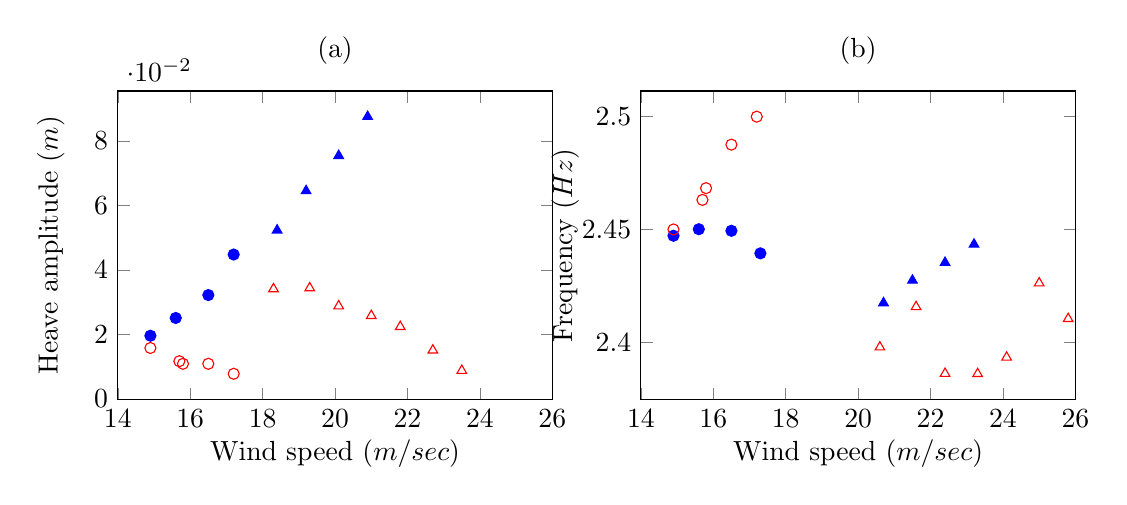
\begin{tikzpicture}
  \begin{groupplot}[group style={group size=2 by 1,horizontal sep=32pt,every plot/.style={xmin=14,xmax=26},xlabels at=edge bottom,vertical sep=30pt},width=7.1cm,height=5.5cm,xlabel={Wind speed ($m/sec$)},ylabel={Heave (m)},x label style={at={(0.5,-0.1)}},	scatter/classes={%
  		a={mark=*,mark size=2pt,blue},%
  		b={mark=o,mark size=2pt,red}},%
    ,legend style={at={(0.33,0.95)}}]

  \nextgroupplot[title=(a),ylabel={Heave amplitude ($m$)},y label style={at={(-0.1,0.5)}}]
  \addplot [mark=*,only marks,%
		mark size=2pt,blue]
    table {
  x     y
  14.9000    0.0196
  15.6000    0.0251
  16.5000    0.0322
  17.2       0.04477
  	};\label{q3}
\addplot [mark=o,only marks,%
    mark size=2pt,red]
    table {
  x     y
  14.9000    0.0158
  15.7000    0.0117
  15.8000    0.0109
  16.5000    0.0109
  17.2000    0.0078
      };\label{q4}

\addplot [mark=triangle*,only marks,%
    mark size=2pt,blue]
    table {
  x     y
  18.4000 0.0523
  19.2000 0.0645
  20.1000 0.0754
  20.9000 0.0875
    };\label{q5}

\addplot [mark=triangle,only marks,%
          mark size=2pt,red]
          table {
  x     y
  18.3000 0.0341
  19.3000 0.0344
  20.1000 0.0288
  21.0000 0.0258
  21.8000 0.0224
  22.7000 0.0151
  23.5000 0.0088
        };\label{q6}
  \nextgroupplot[title=(b),ylabel={Frequency ($Hz$)},y label style={at={(-0.12,0.5)}}]
  \addplot [scatter,only marks,%
		scatter src=explicit symbolic]
    table[meta=label] {
  x     y      label
  14.9000    2.4472 a
  15.6000    2.4501 a
  16.5000    2.4494 a
  17.3000    2.4394 a
  14.9000    2.4500 b
  15.7000    2.4631 b
  15.8000    2.4683 b
  16.5000    2.4876 b
  17.2000    2.5000 b
  	};

\addplot [mark=triangle*,only marks,%
  mark size=2pt,blue]
  table {
  x     y
  20.7000    2.4174
  21.5000    2.4274
  22.4000    2.4353
  23.2000    2.4434
  };

\addplot [mark=triangle,only marks,%
            mark size=2pt,red]
            table {
  x     y
  20.6000    2.3978
  21.6000    2.4157
  22.4000    2.3861
  23.3000    2.3860
  24.1000    2.3933
  25.0000    2.4262
  25.8000    2.4104
};

  \end{groupplot}

  \end{tikzpicture}
  \centering
\caption{CBC results (a) Heave amplitude of LCO ($m$), (b) Frequeny of LCO ($Hz$). (\ref{q3}) is measured stable LCO of system 1 and (\ref{q4}) is the measured unstable LCO of system 1, (\ref{q4}) is measured stable LCO of system 2 and (\ref{q5}) is the measured unstable LCO of system 2.}
\label{f:5}
\end{figure}

CBC results can be used to check if the identified linear model captures important bifurcation characteristics such as flutter speed and flutter frequency. The verification of the linearized model can be done by comparing flutter speed and flutter frequency with the CBC results. Under \asref{a1}, the square of LCO amplitude is proportional to the control parameter. Therefore, flutter speed can be estimated from the linear regression of the square of LCO amplitude crosses zero (\Fref{f:6} (a)), and flutter frequency can be estimated from the relation between the control parameter and the frequency  which is a linear function if we truncate the normal form to the third order (\Fref{f:6} (b)).

\begin{figure}
  \pgfplotsset{every axis title/.append style={at={(0.5,0.95)}}}
  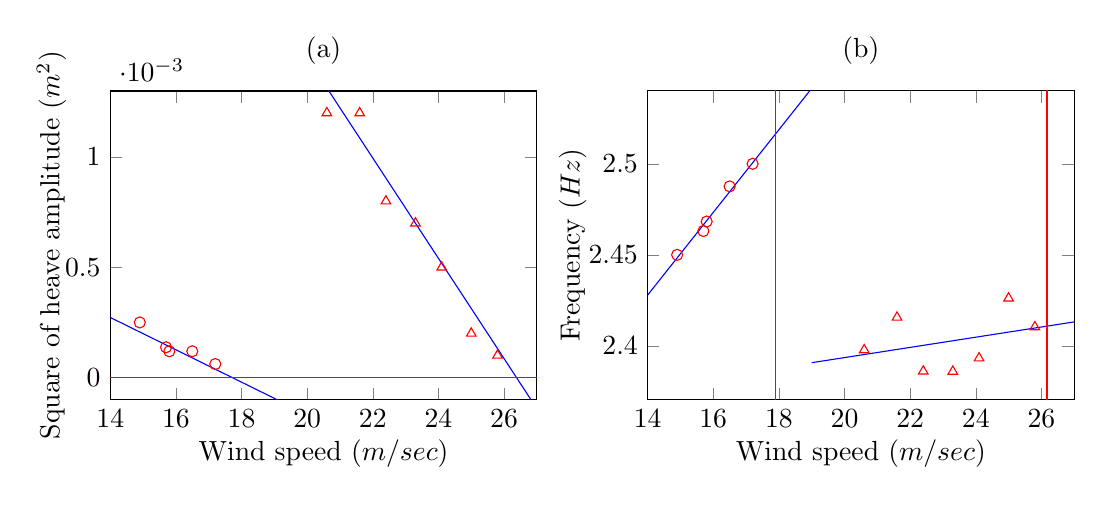
\begin{tikzpicture}
  \begin{groupplot}[group style={group size=2 by 1,horizontal sep=40pt,every plot/.style={xmin=14,xmax=27},xlabels at=edge bottom,vertical sep=30pt},width=7cm,height=5.5cm,xlabel={Wind speed ($m/sec$)},ylabel={Heave (m)},x label style={at={(0.5,-0.1)}}]

  \nextgroupplot[title=(a),ymax=0.0013,ymin=-0.0001,ylabel={Square of heave amplitude ($m^2$)},y label style={at={(-0.08,0.5)}}]

  \addplot [
      domain=14:21,
      samples=10,
      color=blue,
  ]
  {-7.3408e-05*x+0.0013};
  \draw [red] (axis cs:13,0)--(axis cs:19,0);

  \addplot [only marks,mark=o,color=red]
      table {
      X     Y
      14.9	0.00024964
      15.7	0.00013689
      15.8	0.00011881
      16.5	0.00011881
      17.2	0.00006084
      };

  \addplot [
      domain=19:27,
      samples=10,
      color=blue,
      ]
      {-2.2748e-04*x+0.006};
      \draw [red] (axis cs:13,0)--(axis cs:27,0);

  \addplot [only marks,mark=triangle,color=red]
      table {
      X     Y
      20.6000 0.0012
      21.6000 0.0012
      22.4000 0.0008
      23.3000 0.0007
      24.1000 0.0005
      25.0000 0.0002
      25.8000 0.0001
          };

  \nextgroupplot[title=(b),ymax=2.54,ylabel={Frequency ($Hz$)},y label style={at={(-0.12,0.5)}},legend style={at={(0.47,0.98)}}]
  \addplot [
      domain=14:19,
      samples=10,
      color=blue,
  ]
  {0.0227*x+2.1101};
  \draw [red] (axis cs:17.9,2)--(axis cs:17.9,3);
  %Here the blue parabloa is defined
  \addplot [only marks,mark=o,color=red]
      table {
      X     Y
      14.9	2.45
      15.7	2.4631
      15.8	2.4683
      16.5	2.4876
      17.2	2.5
      };
  \addplot [
      domain=19:27,
      samples=10,
      color=blue,
      ]
  {0.0028*x+2.3376};
      \draw [red] (axis cs:26.17,2)--(axis cs:26.17,3);
  \addplot [only marks,mark=triangle,color=red]
      table {
      X     Y
      20.6000    2.3978
      21.6000    2.4157
      22.4000    2.3861
      23.3000    2.3860
      24.1000    2.3933
      25.0000    2.4262
      25.8000    2.4104
              };

  \end{groupplot}

  \end{tikzpicture}
  \centering
\caption{Estimation of flutter properties based on normal form (a) flutter speed estimation, (b) flutter frequeny estimation. (\ref{q1}) is linear regression curve of measured square of heave amplitude, and (\ref{q4}) is measured response of system 1, and (\ref{q6}) is measured response of system 2.}
\label{f:6}
\end{figure}

Estimated futter speed from the model is 17.96 $m/s$ and measured futter speed is 17.89 $m/s$ for system 1. For system 2, estimated flutter speed from the model is 23.95 $m/s$ and measured flutter speed is 26.17 $m/sec$. Estimated futter frequency from the model is 2.46 $Hz$ measured flutter frequency is 2.51 $Hz$ for system 1. For system 2, estimated flutter frequency from the model is 2.41 $Hz$ and measured flutter frequency is 2.41 $Hz$. These results shows identified linearized dynamical model is sufficiently accurate in the sense of predicting flutter speed and frequency from the mathematical model.

\subsubsection{Nonlinear parameter estimation of the flutter rig}\label{nonlinear}

If $U=U_f-\mu$ is inserted to \Eref{eq:2-6}, where $U_f$ is the flutter speed and $\mu=U_f-U$, \Eref{eq:2-6} has Hopf bifurcation at $\mu=0$. First, \Eref{eq:2-6} should be expressed in the form of \Eref{eq:2} by adding $\dot \mu=0$ to the equation of motion. Then, 3-dimensional center manifold and reduced dynamics on the center manifold can be computed from \Eref{eq:3}. Julia \cite{bezanson2017julia} package is developed to compute the center manifold and normal form in this research, and developed code to compute center manifold and normal form can be found in the package \cite{hopfNF}.

Now, SNF of \Eref{eq:2-6} for amplitude can be computed using the coefficients of reduced dynamics for system 1 as
\begin{align}\label{eq:2-11}
\frac{dR}{dt}=&8.8\times 10^{-3}\mu R+(- 7.10 \times 10^{-6}  k_{\alpha 3} + 2.33 \times 10^{-8} k_{\alpha 2}^2)R^3,
\end{align}

\noindent and for system 2 as

\begin{align}\label{eq:2-11-2}
\frac{dR}{dt}=&6.8\times 10^{-3}\mu R+(- 4.6 \times 10^{-6}  k_{\alpha 3} + 1.28 \times 10^{-8} k_{\alpha 2}^2)R^3,
\end{align}

\noindent Amplitude of LCO is now function of nonlinear parameters $k_{\alpha2}$, $k_{\alpha3}$, and $\mu$ which is a nonzero fixed point of \Eref{eq:2-11}, \Eref{eq:2-11-2}. Nonlinear parameter vector $\theta_n=[k_{\alpha2}$, $k_{\alpha3}]^T$ can be identified by solving \Eref{NSI-3} where the numerical code is included in Julia package \cite{hopfNF}. For system 1, optimized value of $\theta_n$ is

\begin{align}\label{eq:2-15}
k_{\alpha2}=3010.0 \: Nm, \; k_{\alpha3}=3000.1 \: Nm.
\end{align}

\noindent and for system 2 as

\begin{align}\label{eq:2-15-2}
k_{\alpha2}=2917.2 \: Nm, \; k_{\alpha3}=519.0 \: Nm.
\end{align}

Computed amplitude via numerical continuation, and measured amplitude are compared for the validation, which is presented in \Fref{f:8}. Numerical continuation results are carried out with coco \cite{dankowicz2013recipes} using identified parameters. $x$-axis of the measured responses are shifted by the difference of the flutter speed between the model and the measured result to compare the amplitude of LCO as a function of $\mu=U-U_f$. Measured and computed heave amplitude from the numerical continuation is in good agreement. There are several aspects to improve the identified model; however, proposed system identification method-- linearized model parameters identification from linear state-space model and nonlinear parameters identification using spectral methods-- can successfully build a mathematical model that capture bifurcation behavior in combination with the proposed CBC scheme.

Less accurate agreement for fold point and the stable upper branch is presumably due to inaccuracy of aeroelastic model of unsteady flutter equation in large response. To increase the accuracy of the parameter identification, more sophisticated aeroelastic model should be considered. However, building the mathematical model that captures the exact fold point and the stable branch is beyond the scope of this research.

\begin{figure}
  \pgfplotsset{every axis title/.append style={at={(0.5,0.95)}}}
  \begin{tikzpicture}
  \begin{groupplot}[group style={group size=2 by 1,horizontal sep=40pt,every plot/.style={ymax=0.09,ymin=0},xlabels at=edge bottom,vertical sep=30pt},width=7.1cm,height=5.5cm,xlabel={Wind speed ($m/sec$)},ylabel={Heave (m)},x label style={at={(0.5,-0.1)}},scatter/classes={%
  		a={mark=*,mark size=2pt,blue},%
  		b={mark=o,mark size=2pt,red}},legend style={at={(0.33,0.95)}}]

  \nextgroupplot[title=(a),xmin=13.5,xmax=18,ylabel={Heave amplitude ($m$)},y label style={at={(-0.05,0.5)}},legend style={at={(0.35,0.98)}}]

  \addplot [no marks,color=blue]
        table [x=a, y=b, col sep=comma] {./Data/Data_8-1.csv};\label{p1}
  %Here the blue parabloa is defined

  \addplot [only marks,color=blue,mark size=2pt%
	]
    table[] {
  x     y
  14.9000    0.0196
  15.6000    0.0251
  16.5000    0.0322
  17.3000    0.0448
  	};\label{p3}
    \addplot [only marks,%
      mark size=2pt,red,mark=o]
      table {
    x     y
    14.9000    0.0158
    15.7000    0.0117
    15.8000    0.0109
    16.5000    0.0109
    17.2000    0.0078
      };\label{p4}
  \nextgroupplot[title=(b),xmin=17,xmax=24.5,ylabel={Heave amplitude ($m$)},y label style={at={(-0.12,0.5)}}]

  \addplot [no marks,color=blue]
        table [x=a, y=b, col sep=comma] {./Data/Data_8-2.csv};

  \addplot [scatter,only marks,%
		scatter src=explicit symbolic]
    table[meta=label] {
  x     y      label
  18.4000 0.0523 a
  19.2000 0.0645 a
  20.1000 0.0754 a
  20.9000 0.0875 a
  18.3000 0.0341 b
  19.3000 0.0344 b
  20.1000 0.0288 b
  21.0000 0.0258 b
  21.8000 0.0224 b
  22.7000 0.0151 b
  23.5000 0.0088 b
  	};

  \end{groupplot}

  \end{tikzpicture}
  \centering
\caption{ Comparison between measured and Computed amplitude of limit cycle. (a) Heave amplitude of system 1 (b) Heave amplitude of system 2. (\ref{p1}) is computed amplitude by numerical continuation, (\ref{p3}) is measured stable limit cycle, and (\ref{p4}) is measured unstable limit cycle.}
\label{f:8}
\end{figure}

\section{Conclusion}
CBC scheme for stabilizing unstable LCOs near Hopf bifurcation is developed. A dynamical system with CBC can be simplified to a Hopf bifurcation with single harmonic forcing if weakly nonlinear transformation and small amplitude response is assumed during normal form derivation. Input-output map of CBC for Hopf bifurcation can be defined as a one-dimensional map if phase-locking between the control target and the response is forced by the real-time controller. Therefore, finding a noninvasive periodic solution is equivalent to finding a zero solution of the control error function. Developed CBC scheme is applied to a flutter rig with two different spring plate. These results can be applied to verify the identified linearized dynamical model and used as an identification tool of the grey-box model of a self-excited system.

To apply PP-CBC to more general problems, phase locking scheme for multiharmonic response should be developed. Also, a methodology to overcome the influence of the measurement noise should be considered to improve the accuracy of the CBC results. \vskip6pt


\enlargethispage{20pt}

\dataccess{Insert data access text here.}

\aucontribute{All authors contributed to the formation and fundamental concepts of the research. D.A.W.B. developed the PP-CBC scheme and the exprimental setup. L.R. assisted on experimental data analysis and system identification. All authors contributed to the preparation of the manuscript.}

\competing{We have no competing interests}

\funding{Insert funding text here.}

\ack{Insert acknowledgment text here.}

\begin{appendices}
\gdef\thesection{Appendix \Alph{section}}

\section{SNF of Hopf bifurcation} \label{ap0}
Near identity transformation
\(x=h(u,\bar{u},\nu))=u+\sum_k h_k(u,\bar{u},\nu)\), time rescailing \(t=T(u,\bar{u},\nu,\tau)\) and parameter rescailing \(\lambda=p(\nu)\) can be expressed in power series as

\begin{align}\label{eq:6}
  \begin{split}
    h_k &=\sum_{j+l+m=k}(c_{ijkm}+\textrm{i}c_{2jlm}u^j\bar{u}^l \nu^m),\\
    t &=\Big(1+\sum_{k=1}\sum_{j+m=k}t_{jm}(u+\bar{u})^j\nu^m\Big)\tau,\\
    \lambda &=\nu+\sum_{j=2}p_j \nu^j.
  \end{split}
\end{align}

\noindent Coefficients of \Eref{eq:6} can be computed recursively \cite{yu2002simplest} by eliminating noncritical terms of \Eref{eq:4}. Coefficients of \Eref{eq:5} can be derived with coefficients of original coordinate as $\alpha_1=\vec{a}_{1101}$, $\beta_1=1$, $\alpha_2=a_{1210}-a_{1200}a_{2110}-a_{2200}a_{1110}$, and  (see \cite{yu2002simplest} for coefficients of $g_k$, $h_k$, $t_{jm}$, and $p_j$).

\end{appendices}

%%%%%%%%%% Insert bibliography here %%%%%%%%%%%%%%

\bibliography{ref}
\bibliographystyle{vancouver}
\end{document}



\end{document}
